% General Paper Template created by Adam Green
% Last revised 2/20/18

\documentclass[12pt]{article}

%%%%%%%%%%%%%%%%%%%%%%%%%%
% Standard Packages
%%%%%%%%%%%%%%%%%%%%%%%%%%
\usepackage{amsmath,amsfonts,amsthm,amssymb}
\usepackage[margin = 2cm]{geometry}


%%%%%%%%%%%%%%%%%%%%%%%%%%
% Graphical Packages
%%%%%%%%%%%%%%%%%%%%%%%%%%
\usepackage{graphicx}
\usepackage{subfig}
\usepackage{float}
\usepackage{tikz}
\usepackage{wrapfig}
% Syntax: \begin{wrapfig}[lineheight]{position}{width}

%\usepackage{tikz-3dplot}
%\usepackage{pgfplots}

\graphicspath{{Figures/}} % set directory for figures

%%%%%%%%%%%%%%%%%%%%%%%%%%
% Colors
%%%%%%%%%%%%%%%%%%%%%%%%%%
\usepackage{xcolor}

\definecolor{myblue1}{RGB}{76, 142, 185}
\definecolor{myblue2}{RGB}{25, 100, 126}
\definecolor{myblue3}{RGB}{41, 110, 180}

\definecolor{mygreen1}{RGB}{88,165,87}
\definecolor{mygreen2}{RGB}{91,165,98}

\definecolor{myred1}{RGB}{221, 28, 26}
\definecolor{mypurple}{RGB}{122,48,108}


%%%%%%%%%%%%%%%%%%%%%%%%%%
% Table and Array Packages
%%%%%%%%%%%%%%%%%%%%%%%%%%
\usepackage{tabu}
\usepackage{booktabs}


%%%%%%%%%%%%%%%%%%%%%%%%%%
% Citation Packages
%%%%%%%%%%%%%%%%%%%%%%%%%%
\usepackage{hyperref}
\hypersetup{allcolors = myblue1,
			allbordercolors = myblue1, 
			filecolor = myblue1, 
			linkbordercolor = myblue1,
			urlbordercolor = white
    		}

\usepackage{cleveref}
\crefname{equation}{Eqn.}{Eqns.}
\crefname{figure}{Fig.}{Figs.}
\crefname{table}{Tab.}{Tabs.}

%\usepackage{caption}
%	\captionsetup{format = , justification= }

%%%%%%%%%%%%%%%%%%%%%%%%%%
% Text Formatting packages
%%%%%%%%%%%%%%%%%%%%%%%%%%
\usepackage{multicol}
\usepackage{parskip} 
\usepackage{indentfirst} 
	\setlength{\parindent}{0.75cm}
\usepackage{fancyhdr}
%	\pagestyle{fancy}
\usepackage{enumerate}
\usepackage{wrapfig}
\usepackage{lipsum}
\usepackage{xhfill}

%%%%%%%%%%%%%%%%%%%%%%%%%%
% Custom Commands
%%%%%%%%%%%%%%%%%%%%%%%%%%
% Red marks to get attention
\newcommand{\red}[1]{\textbf{\textcolor{myred1}{#1}}} % Red Text
\newcommand{\redmark}{\textcolor{myred1}{\rule{3.5mm}{3.5mm} }} % Red Dash
\newcommand{\redline}{\noindent\xhrulefill{myred1}{3pt}} % Red Rule
\newcommand{\whitefill}{\textcolor{white}{\rule{\textwidth}{2.5pt} } }


% Lowercase captial letters
\newcommand{\scap}[1]{\textsc{\MakeLowercase{#1}}} % Makes caps small so it doesnt SHOUT


% Math commands, first and second order partials, Laplacian
\newcommand{\evaluate}{\Bigr\rvert}
\newcommand{\ppd}[1]{\frac{\partial}{\partial#1}}
\newcommand{\ppsd}[1]{\frac{\partial^2}{\partial #1^2}}
\newcommand{\ppnd}[2]{\frac{\partial #1}{\partial #2}}
\newcommand{\ppsnd}[2]{\frac{\partial^2 #1}{\partial #2^2}}
\newcommand{\lap}{\nabla^2}

% Quantum bra- ket- commands
\newcommand{\bra}[1]{\langle #1 |}
\newcommand{\ket}[1]{| #1 \rangle}
\newcommand{\bracket}[2]{\langle #1 | #2 \rangle}

% Redfine equation and figure references to include "Eqn. ()" and "Fig. _"
%\newcommand{\figref}[1]{Fig.\ \ref{#1}}
%\let\originaleqref=\eqref
%\renewcommand{\eqref}{Eqn.\ \originaleqref}


% Custom Matrix Spacing
% Syntax: \begin{matrix}[scale]
\makeatletter
\renewcommand*\env@matrix[1][\arraystretch]{%
	\edef\arraystretch{#1}%
	\hskip -\arraycolsep
	\let\@ifnextchar\new@ifnextchar
	\array{*\c@MaxMatrixCols c}}
\makeatother


% Email Commands: Taken from Flip
\newcommand{\email}[1]{\href{mailto:#1}{\textcolor{mygreen1}{#1}}}

% Institution Environment: Taken From Flip
\newenvironment{institutions}[1][2em]{\begin{list}{}{\setlength\leftmargin{#1}\setlength\rightmargin{#1}}\item[]}{\end{list}}

% Link to external webpage
\newcommand{\link}[1]{\href{#1}{\textcolor{mygreen1}{\texttt{#1}}}}


%%%%%%%%%%%%%%%%%%%%%%%%%%%%
% Document Specific Commands
%%%%%%%%%%%%%%%%%%%%%%%%%%%%
\newcommand{\RbEF}{$^{85}\text{Rb}$ }
\newcommand{\RbES}{$^{87}\text{Rb}$ }
\usepackage{stackengine}
\usepackage{bm}
%\usepackage{romannum}

\begin{document}
	%%%%%%%%%%%%%%%%%%%%%%%%%%%
	% Title
	%%%%%%%%%%%%%%%%%%%%%%%%%%%	
	\begin{center}
		
		{\LARGE \bf Hyperfine and Zeeman Splitting of \RbEF and \RbES}\\

		\vspace{0.5cm}
		
		\textbf{Adam Green}, \textbf{Guillermo Acuna}\\
		
		\texttt{\footnotesize \email{agree019@ucr.edu}},
		\texttt{\footnotesize \email{gacun002@ucr.edu}}
		
		\vspace{0.5cm}
		
		
		\begin{institutions}[2.25cm]
			\footnotesize
			{\it 
				Department of Physics \& Astronomy, 
				University of  California, Riverside, 
				CA 92521	    
			}    
		\end{institutions}
		
		\vspace{0.5cm}
		
	\end{center}
	
	%%%%%%%%%%%%%%%%%%%%%%%%%%%
	% Abstract
	%%%%%%%%%%%%%%%%%%%%%%%%%%%	
	\vspace{0.5cm}
	\begin{abstract}
		In this experiment, we study the hyperfine splitting and Zeeman effect for naturally occurring Rubidium using saturated absorption spectroscopy. For $^{85}\text{Rb}$, we measure the splitting between the $F=2$ and $F=3$ states to be $3320 \ \text{MHz} \pm 117 \ \text{MHz}$. For $^{87}\text{Rb}$, we determine the splitting between the $F=1$ and $F=2$ state to be $7390 \ \text{MHz} \pm 117 \ \text{MHz}$. We provide quantitative energy level diagrams for both isotopes of Rubidium. Further, upon the application of an external magnetic field, we measure the splitting between the hyperfine transitions. We provide an analysis of Zeeman splitting vs magnetic field strength and we determine the Land\'e g-factor to be $g_F = 0.307 \pm 0.0103$.
	\end{abstract}
	
	\tableofcontents
	
	\section{Introduction}
	The ground states of Hydrogen and Rubidium have effectively the same electron configuration. Hydrogen consists of a single 1s electron while Rubidium consists of a closed shell plus a single 5s electron. This indicates that their spectra should share similar features. Solving the Schr\"odinger equation yields an energy spectra dependent on the principal quantum number ``$n$'' which contains $n^2$ degeneracies.
	
% Energy Level Diagram for Hydrogen
	\begin{wrapfigure}{R}{0.5\textwidth}
		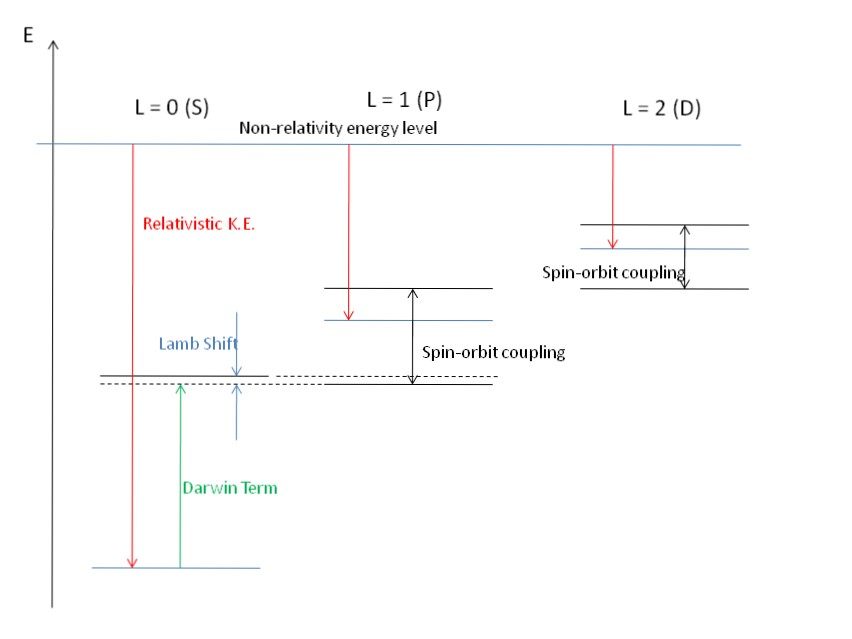
\includegraphics[width=0.5\textwidth]{Fine_Structure/HydrogenFineStructure1.jpg}
		\caption{Qualitative energy level diagram displaying the fine structure corrections for Hydrogen}
		\label{HydrogenFine}
	\end{wrapfigure}


	%Long Version
	These degeneracies in n are resolved when a number of corrective effects are included. The first is a statement that electrons are moving at relativistic speeds which affects their kinetic energy, simply known as the \emph{relativistic kinetic energy} correction. The second two only effect the s-orbital: the \emph{Darwin Term} and \emph{Lamb Shift}. The Darwin term is the smearing out of the Coulomb interaction between the nucleus and electron due to quantum fluctuations. The \emph{Lamb shift} arises from quantum electrodynamic interactions between the electrons and the vacuum. The final correction is known as \emph{spin-orbit coupling}, which arises from interactions between the orbital and spin angular momenta of the election. Collectively, these corrections are referred to as the \emph{fine structure} and are visualized in \cref{HydrogenFine}.
	
	These states are denoted by ``term states'' in the spectroscopic notation $^{2S+1}L_J$, where $L$ is the spectroscopic notation, $S,P,D,F$ for the corresponding orbital angular momentum quantum numbers $L=0,1,2,3$. In this notation, the ground state of the 5s Rb electron is denoted as $^2S_{1/2}$ and the first excited state is denoted $^2P_{3/2}$.
	
	The Fine structure though is still degenerate. To resolve these degeneracies, we must account for one additional effect. If the nucleus has a magnetic moment, denoted by $\vec{I}$, the electron will interact with this magnetic field. This interaction, known as the \emph{Zeeman Effect}, will change the energy of the electron depending on the orientation of its spin. The additional corrections to the fine structure energy levels are known as the \emph{hyperfine structure} corrections. If the hyperfine splitting is much less than the fine structure splitting, then the magnetic quantum number $I=|\vec{I}|$ and orbital angular momentum quantum number $J$ are good quantum numbers. Further, the degeneracy in the fine structure is split according to total the angular momentum $F=I+J$. Note that $F$ takes values between $\{|I-J|, |I-J+1|,...,|I+J|\}$. With respect to the fine structure, the energy levels are split by:
	\begin{equation}
		\label{hyperfineSplitting}
		E = \frac{\gamma}{2}\left[ F(F+1) - I(I+1) - J(J+1) \right]
	\end{equation}
	where $\gamma$ is the hyperfine structure constant.
	
	Rubidium has two naturally occurring isotopes, \RbEF ($72\%$ abundance) with $I=\frac{5}{2}$, and \RbES ($28\%$ abundance) with $I=\frac{3}{2}$. A spectroscopic analysis of naturally occurring Rubidium will contain both isotopes superimposed on top of each other. 
	
	For an atom with magnetic moment $\bm{\mu}$, a magnetic field will perturb it by:
	\begin{equation}
		\Delta E = - \bm{\mu} \cdot \mathbf{B} 
	\end{equation}
	If the magnetic field is weak, the Zeeman splitting is small compared to the hyperfine interactions. In the weak field limit, the Zeeman splitting to first order is given by:
	\begin{equation}
		\Delta E_{\text{weak}} = g_F \mu_B m_F B
		\label{zeemanWeak}
	\end{equation}
	where $g_F \approx g_J \frac{F(F+1)-I(I+1)-J(J+1)}{2F(F+1)}$, $g_J$ is the \emph{Land\'e g-factor}, $\mu_B$ is the \emph{Bhor Magneton}, and $m_F=-F,-F+1,...,F$ is the quantum number for $F_z$. 		
	 
	\section{Experimental Procedure}

%	\subsection{Diode Laser}
%	The basic schematic for the diode laser we use is shown in \cref{diodeLaser}. 
%	
%	\begin{figure}[H]
%		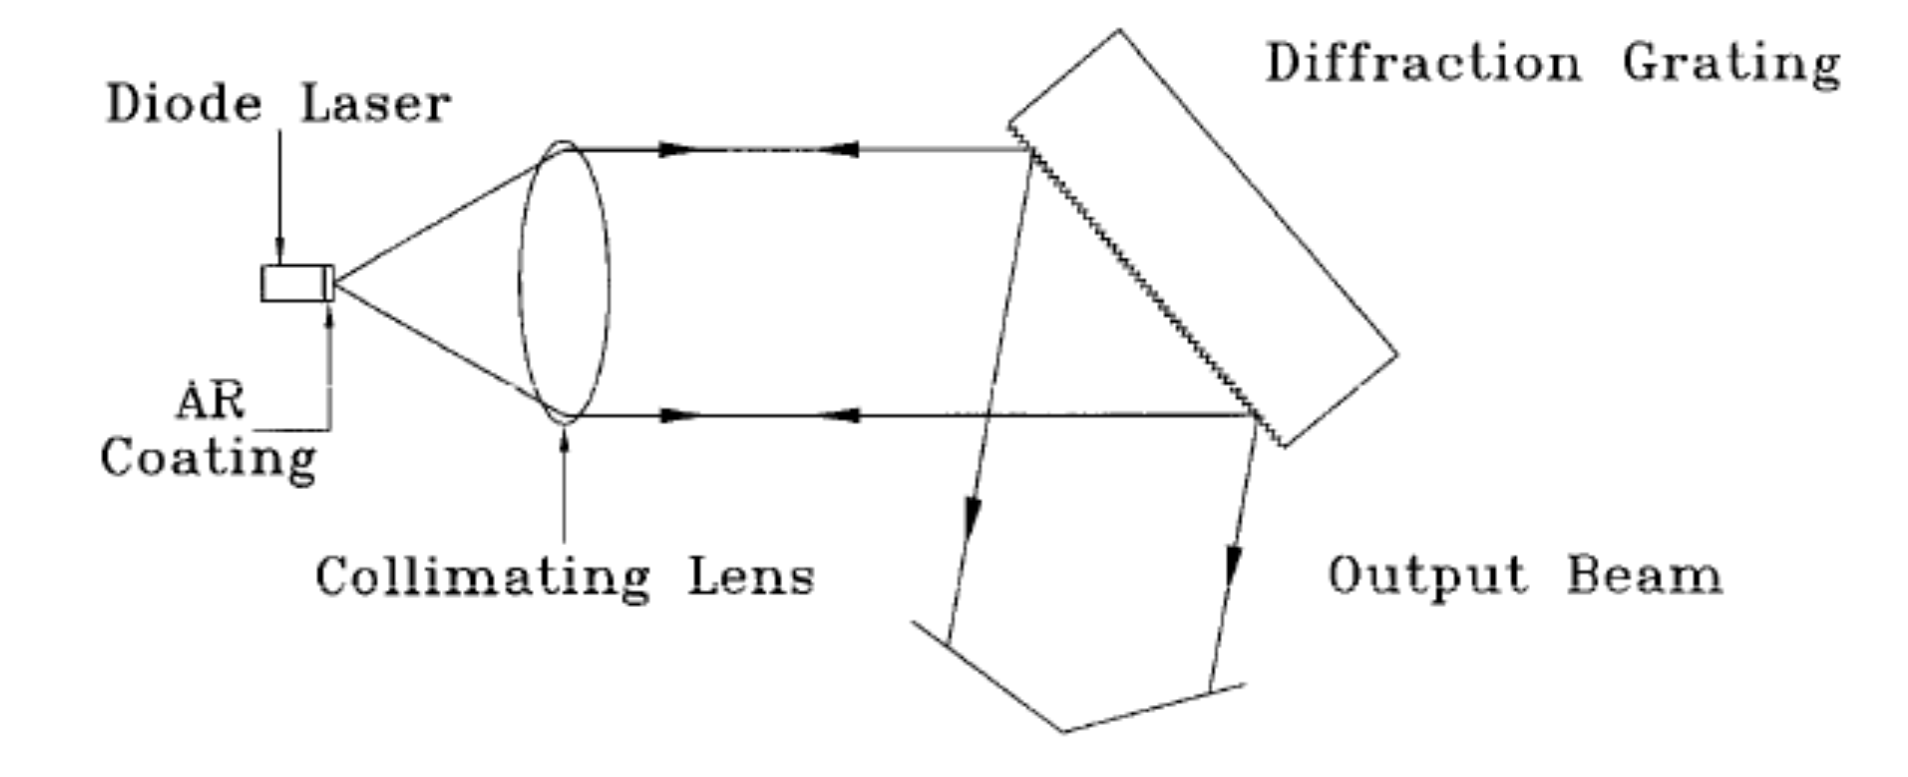
\includegraphics[width=0.4\textwidth]{DiodeLaser/DiodeLaser.PNG}
%		\caption{\red{caption}}
%		\label{diodeLaser}
%	\end{figure}

	% Short Version
	\subsubsection*{Corrective Measures}
	We present here, a brief overview of known complications with saturated absorption spectroscopy and present our corrections to these complications. These complications include mode hopping, Doppler broadening, and crossover resonances within a saturated absorption spectrum. 
	
	Mode hopping occurs when the various components of the laser are changed independently of one another. This results in spectral features which look like absorptions, but are actually due to the frequency selection of the laser, not absorption from a molecule. To correct for mode hopping, the components of the laser must all change simultaneously. This can be accomplished by coupling the amplitude of the laser, the ramp generator, and the piezo controller together as seen in \cref{Setup2}. 
	
	Doppler broadening is a result of atoms in the absorption chamber seeing the beam Doppler shifted into absorption. On the oscilloscope, this will result in a broadened peak around the absorption frequency. One way to eliminate Doppler broadening is performing saturated absorption spectroscopy, where two overlapping beams are sent through the absorption cell.
	
	However, when saturated absorption is performed, the oscilloscope trace will show more absorption peaks than are physically possible. This is because some of the atoms may see only one of the beams Doppler shifted into absorption, and this single-beam absorption will appear as a peak directly in between two transitions. To correct for this effect, we argue that the outside peaks must be genuine transitions, and then look for peaks which lie directly between two other peaks.
	
	\subsubsection*{Saturated Absorption}
%		Saturated absorption spectroscopy reveals the hyperfine structure of Rubidium. More precisely, it resolves very fine absorption lines from a Doppler broadened signal in a two step process. To perform saturated absorption, the beam from the laser must be split into two, one weak and one strong beam. The weak beam, called the \emph{probe} beam, is sent through the Rubidium chamber into the photodiode. The strong beam, called the \emph{pump} beam, is aligned anti-parallel to the probe beam. The first step in saturated absorption involves the pump beam keeping the electrons in the substance perpetually excited. If the pump beam were measured, it would yield a Doppler broadened absorption spectrum just as before. Of those excited electrons, upon interacting with the probe beam, they will undergo stimulated emission. This is the second step in saturated absorption spectroscopy. This stimulated emission only occurs if the atoms see both lasers at an absorption frequency. In other words, if atoms are Doppler shifted into absorption by the pump beam, they will not undergo stimulated emission by the probe beam and thus do not contribute to the fine structure spectrum.

	Saturated absorption spectroscopy reveals the hyperfine structure of Rubidium. More precisely, it resolves very fine absorption lines from a Doppler broadened signal in a two step process. In the first step, a weak \emph{probe beam} is sent through the absorption chamber into the photodiode. The probe beam simply serves to probe the absorption spectrum of the sample. If the spectrum from the probe beam were measured, it would be Doppler broadened just as before. The second step is to overlap a second, stronger \emph{pump beam} anti-parallel with the probe beam. When the two beams are overlapping and anti-parallel, the pump beam keeps the sample in the excited state, and the probe beams generates stimulated emission. However, this stimulated emission only occurs for atoms that see both lasers at an absorption frequency, which allows the fine spectral features to be resolved. In other words, if atoms are Doppler shifted into absorption by the pump beam, they will not undergo stimulated emission by the probe beam and do not contribute to the fine structure spectrum.
	
	\subsubsection*{Calibration}
		
		\begin{wrapfigure}{l}{0.5\textwidth}
			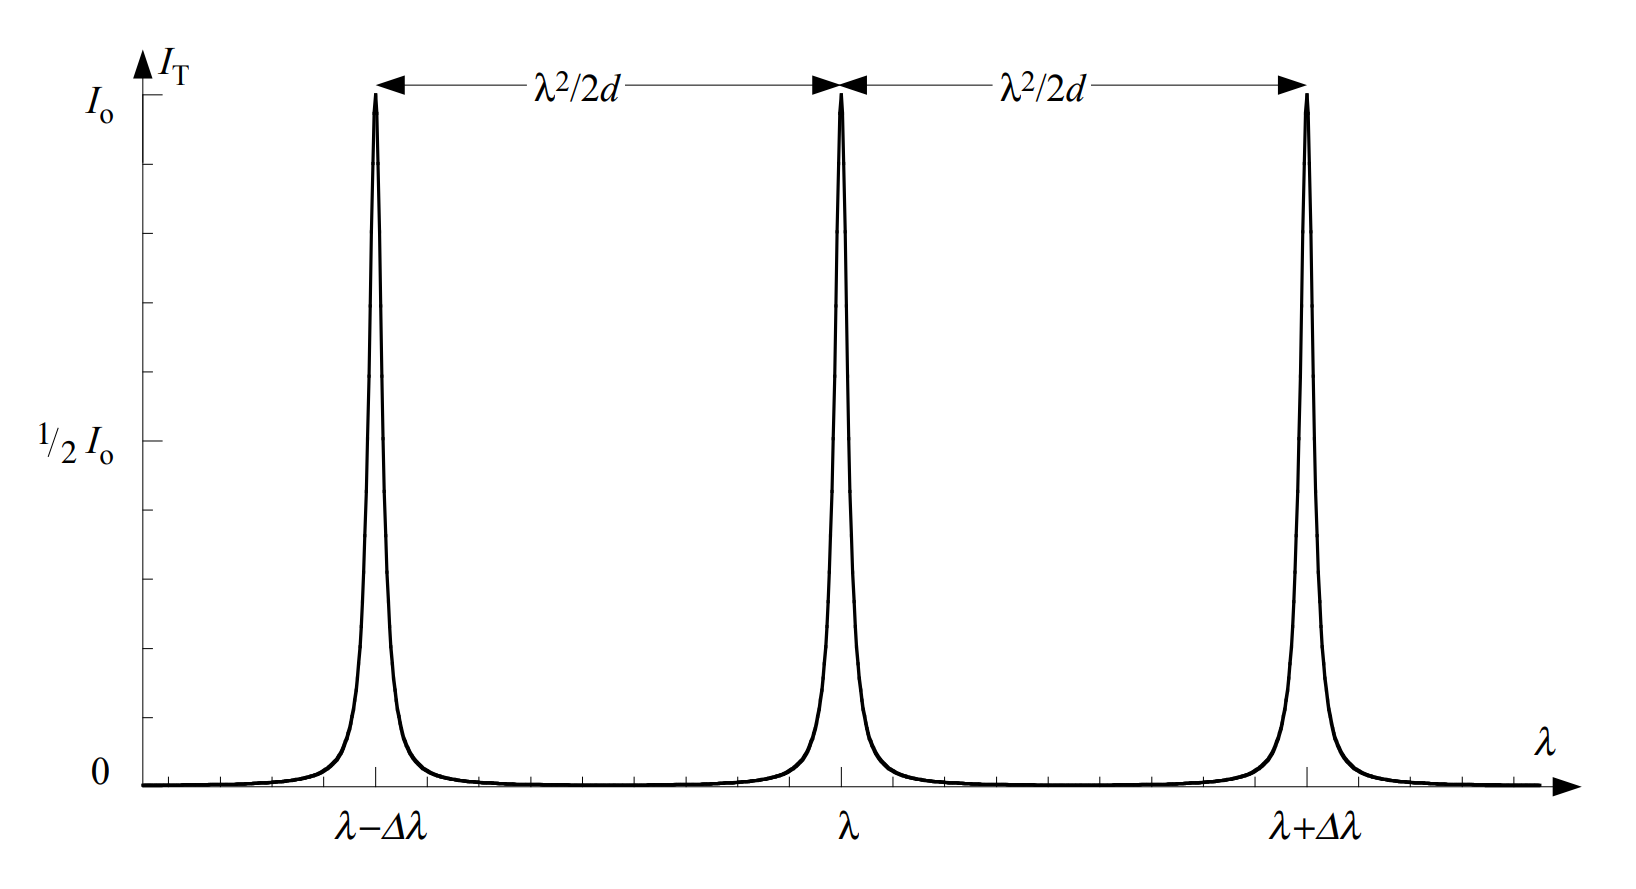
\includegraphics[width=0.5\textwidth]{DiodeLaser/InterferometerScan.png}
			\caption{Representative interferometer oscilloscope trace}
			\label{interferometerScan}
		\end{wrapfigure}
		To quantify the scale of the horizontal axis on the oscilloscope, we must relate the frequency of the laser to the spacing on the oscilloscope. To do this, we use a \emph{Fabry-Perot interferometer}. This is an optical cavity of fixed length which acts as a filter, allowing only certain frequencies to pass through. Upon measuring the transmission intensity from the interferometer, we obtain a spectrum similar to \cref{interferometerScan}. Here, the spacing between each resonant peak is 
		\begin{equation}
			\Delta \lambda = \frac{\lambda^2}{2d}
		\end{equation}
		where $\lambda$ is the frequency of the laser and $d$ is the length of the interferometer. A simple conversion from wavelength to frequency allows us to determine the scale of the horizontal axis on the oscilloscope in terms of laser frequency. This calibration process has already been preformed, and we quote the result of $234 \ \text{MHz/ms}$.
	
	

% Long Version
%	\subsubsection*{Mode Hopping}
%	Mode hopping is an undesirable feature of diode lasers and produces very sharp, discontinuous jumps in spectral scans, see \cref{modeHopping}. The frequency of the laser beam is actually a combination of the frequencies allowed by the various parts of the laser, see \cref{LaserSpectrumCavity}. The parts which contribute to the frequency are $1)$.\ the material of the diode, $2)$.\ the physical size of the internal cavity in the diode, $3)$.\ the diffraction grating and $4)$.\ the separation between the collimating lens and diffraction grating called the external cavity.
%	
%	Here, each of the 4 components helps to ``choose'' the frequency of the laser, the frequency which all components agree on. \red{ In \cref{laserSpectrum} the grating feedback narrows the wavelength down to the neighborhood of $671$ nm. It is further ``fine tuned'' by the external cavity...} In \cref{laserSpectrum}, the contribution from the medium corresponds to a wavelength range from $670.6$ nm to $671.4$ nm. The contribution from the grating feedback selects wavelengths in the neighborhood of $671$ nm, and the contribution from the external cavity acts as the ``fine tuning'' to the wavelength. Mode hops are discreet jumps in the wavelength of the laser due to changes in the various contributions to the wavelength, see \cref{modeHops}.
%	
%	\begin{figure}[H]
%		\centering
%		\subfloat[\red{caption}]{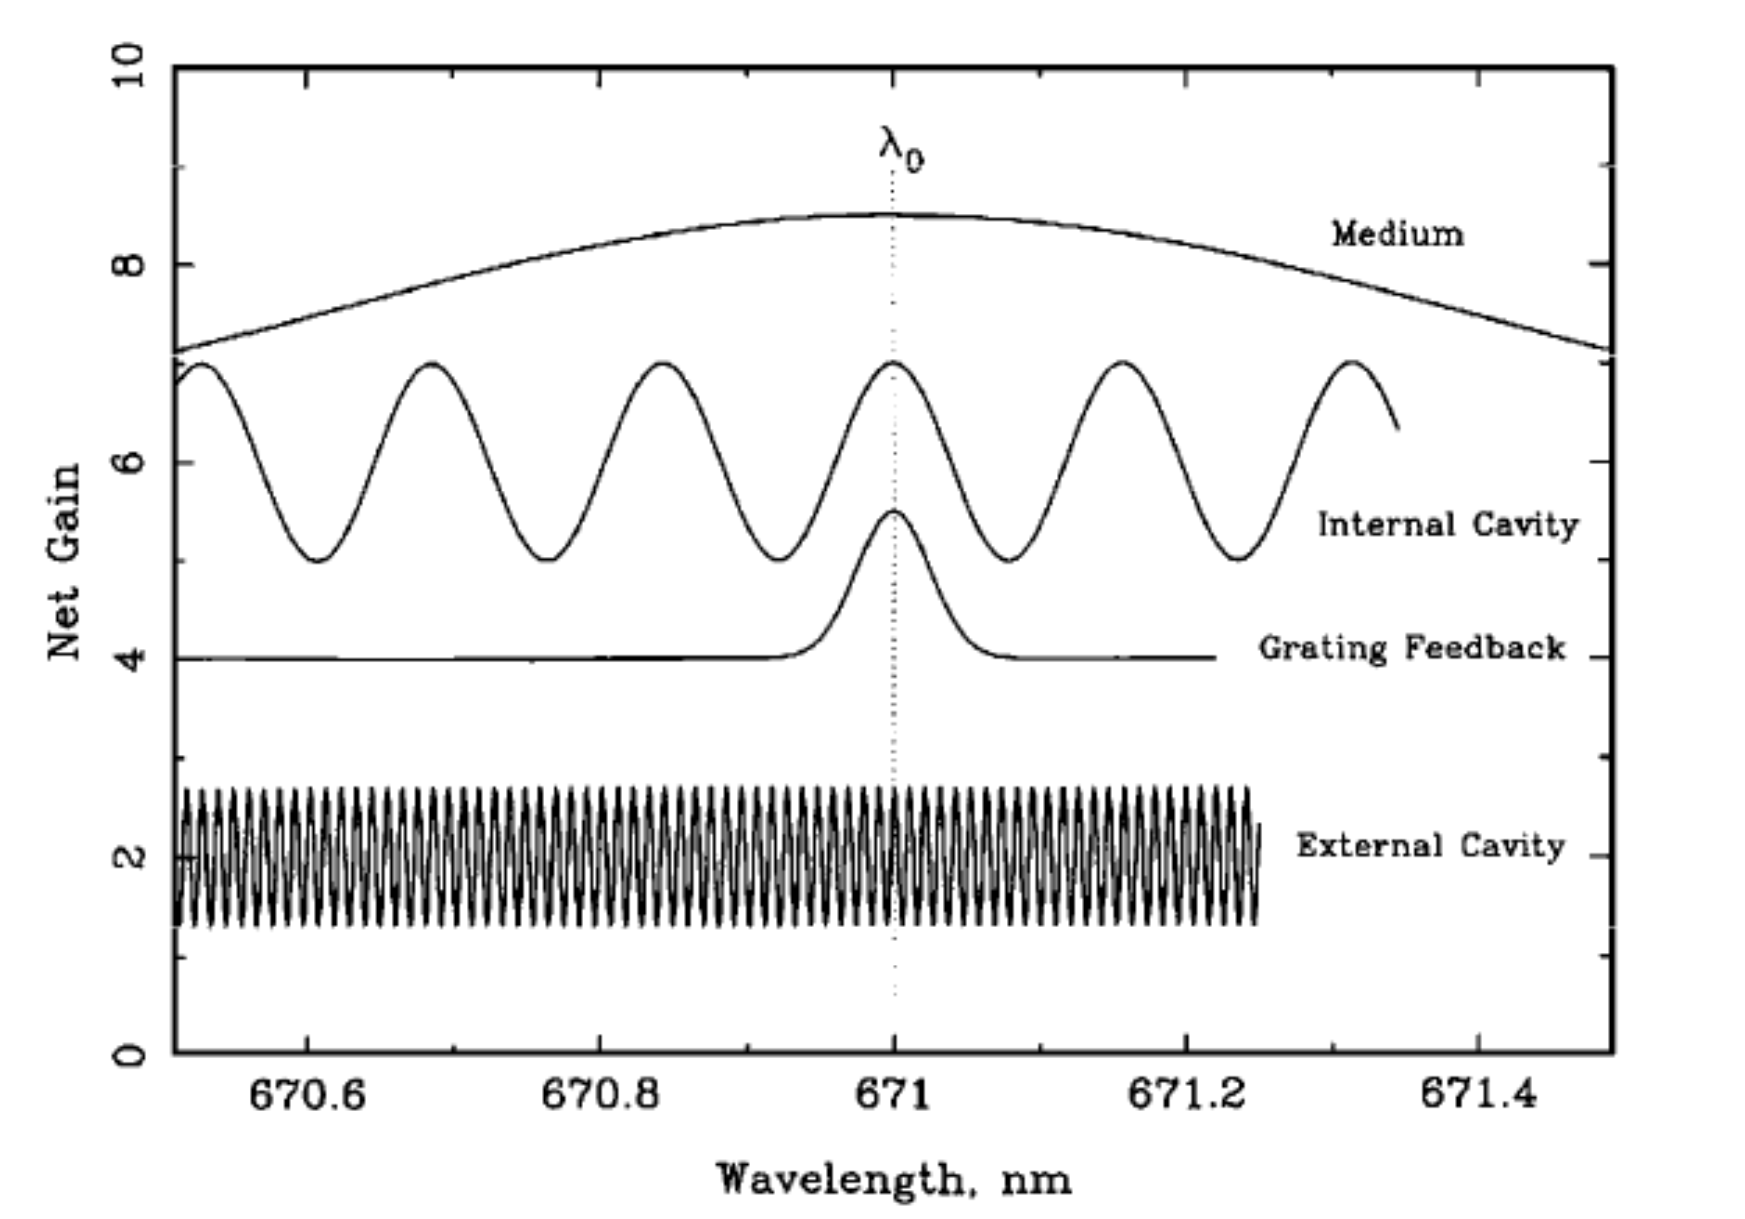
\includegraphics[width=0.4\textwidth]{DiodeLaser/LaserFrequencySpectrum.PNG} \label{laserSpectrum}}
%		\qquad
%		\subfloat[\red{caption}]{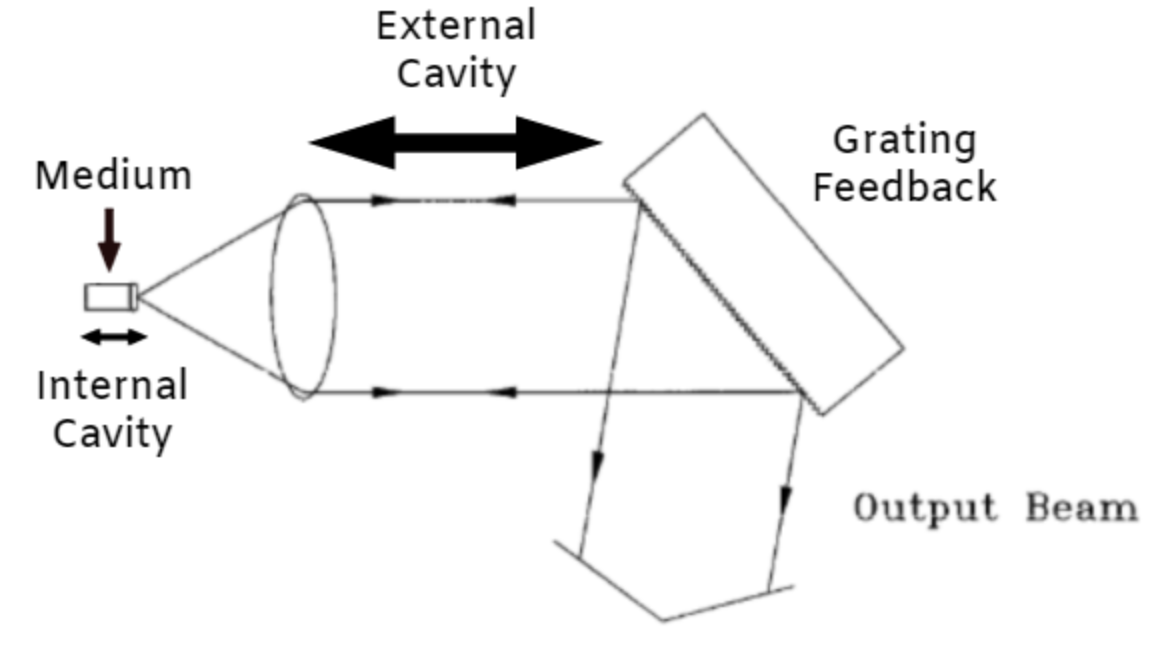
\includegraphics[width=0.45\textwidth]{DiodeLaser/LaserModes1.png} \label{laserCavities} }
%		\caption{\red{caption}}
%		\label{LaserSpectrumCavity}
%	\end{figure}	
%	
%	\subsubsection*{Doppler Broadening}
%	Doppler broadening is the broadening of a signal due to the relative velocity of the atoms interacting with the laser. For this experiment, we are sending a laser through a chamber of naturally occurring Rubidium, referred to as the absorption chamber, and measuring the absorption spectrum. The velocity of the gas inside the chamber follows a Maxwellian distribution, meaning some of the molecules are moving with or against the laser. It is precisely this because of this relative motion that some of the gas molecules see the laser red-shifted, or blue-shifted onto absorption. In other words, some of the atoms in the absorption chamber which are not eligible for absorption are Doppler shifted into absorption, giving a wider range of absorbed frequencies. This ``widening'' of the absorption frequency is what is known as Doppler broadening.
%	
%	\subsubsection*{Saturated Absorption}
%	Saturated absorption spectroscopy reveals the hyperfine structure of Rubidium. More precisely, it resolves very fine absorption lines from a Doppler broadened signal in a two step process. To perform saturated absorption, the beam from the laser must be split into two, one weak and one strong beam. The weak beam, called the \emph{probe} beam, is sent through the Rubidium chamber into the photodiode. The strong beam, called the \emph{pump} beam, is aligned anti-parallel to the probe beam. The first step in saturated absorption involves the pump beam keeping the electrons in the substance perpetually excited. If the pump beam were measured, it would yield a Doppler broadened absorption spectrum just as before. Of those excited electrons, upon interacting with the probe beam, they will undergo stimulated emission. This is the second step in saturated absorption spectroscopy. This stimulated emission only occurs if the atoms see both lasers at an absorption frequency. In other words, if atoms are Doppler shifted into absorption by the pump beam, they will not undergo stimulated emission by the probe beam and thus do not contribute to the fine structure spectrum.
%	
%	\subsubsection*{Crossover Resonance}
%	\begin{wrapfigure}{l}{0.45\textwidth}
%		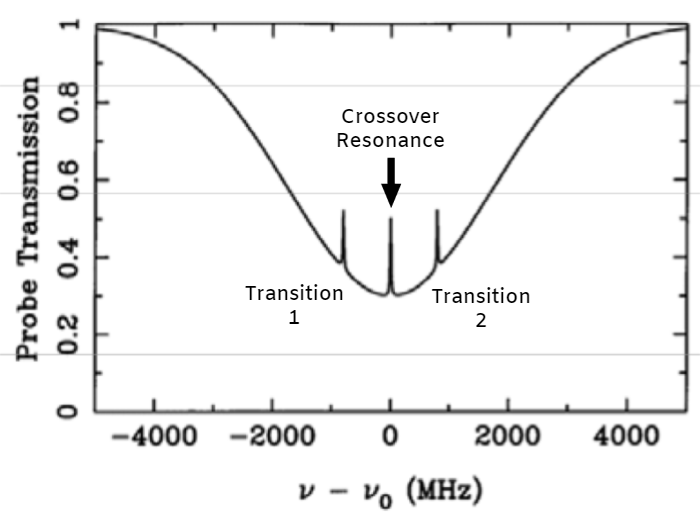
\includegraphics[width=0.4\textwidth]{Crossover/crossoverAnnotated.PNG}
%		\caption{Saturated absorption spectrum for an atom with a single ground state and two excited states displaying a crossover resonance.}
%		\label{crossover}
%	\end{wrapfigure}
%	
%	In saturated absorption measurements, one important effect must be accounted for called \emph{crossover resonances}. If we examine the saturated absorption spectrum of an atom with a single ground state and two excited states, we will find an absorption spectrum similar to \cref{crossover}. Contrary to intuition, we will find three peaks instead of two, corresponding to the two excited states. From the absorption spectrum, crossover resonances appear to represent genuine atomic transitions. However, they arise from interactions of the atoms with the pump and probe beams individually. The hallmark of saturated absorption measurements requires that atoms in the absorption cell see both beams in resonance with atomic transitions. However, there are also atoms which will see only one of the beams in resonance with a transition. So, atoms may absorb due to only the pump or only the probe beam, and this single-beam absorption is what causes crossover resonances. Consequently, one of the distinguishing features of crossover resonances is they will always be directly in between transitions.
%	
%	\subsubsection*{Calibration}
%	
%	\begin{wrapfigure}{l}{0.5\textwidth}
%		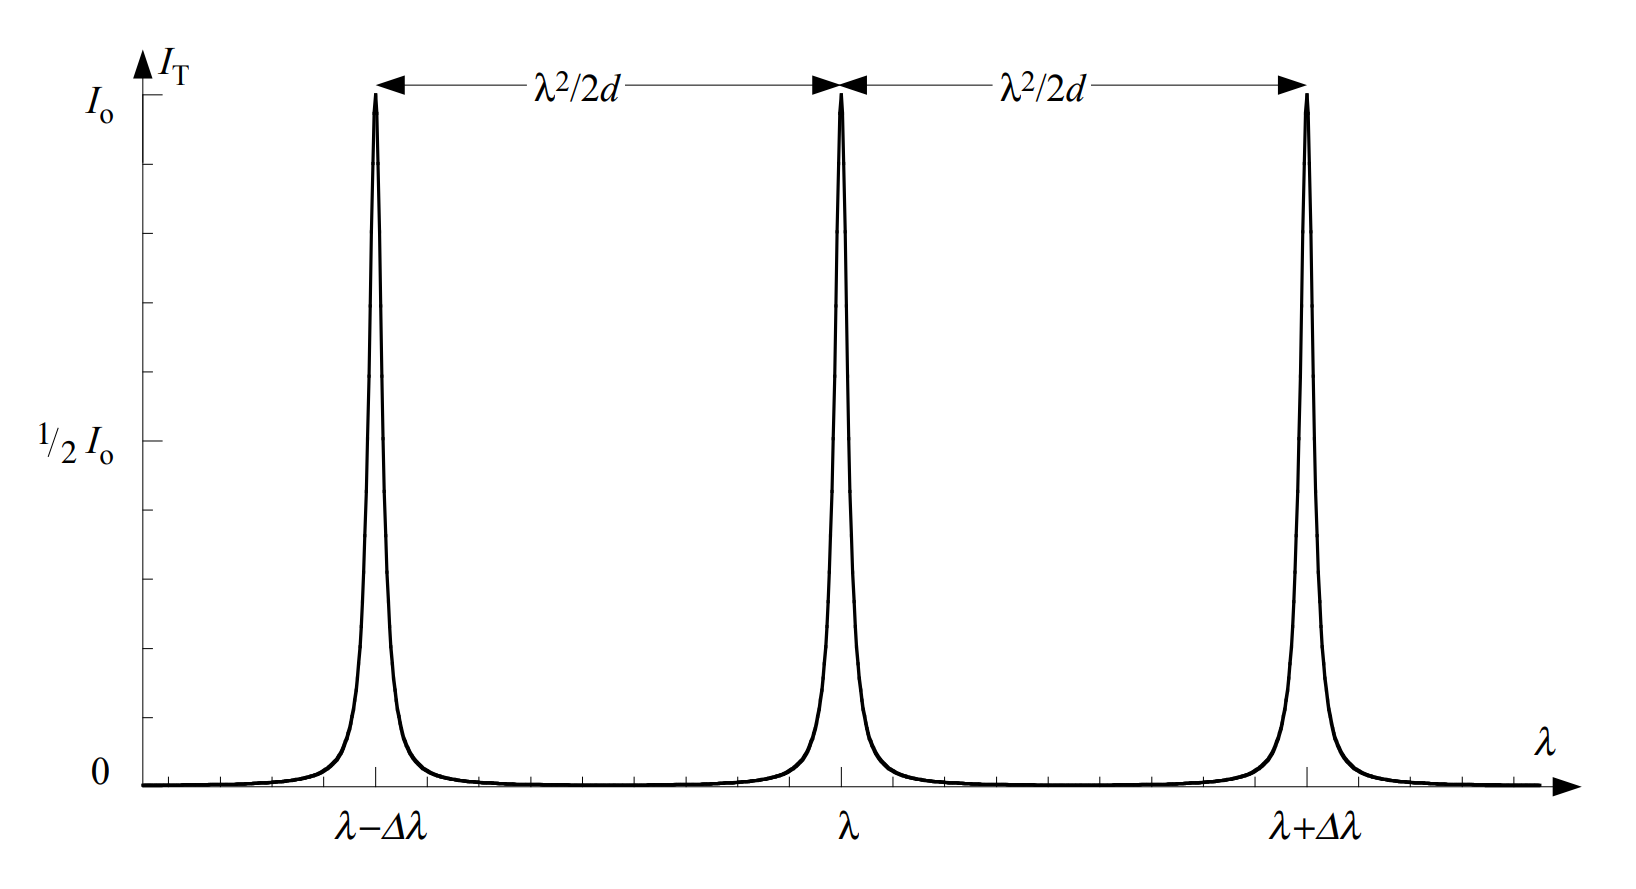
\includegraphics[width=0.5\textwidth]{DiodeLaser/InterferometerScan.png}
%		\caption{Representative interferometer oscilloscope trace}
%		\label{interferometerScan}
%	\end{wrapfigure}
%
%	To quantify the scale of the horizontal axis on the oscilloscope, we must relate the frequency of the laser to the spacing on the oscilloscope. To do this, we use a \emph{Fabry-Perot interferometer}. This is an optical cavity of fixed length which acts as a filter, allowing only certain frequencies to pass through. Upon measuring the transmission intensity from the interferometer, we obtain a spectrum similar to \cref{interferometerScan}. Here, the spacing between each resonant peak is 
%	\begin{equation}
%		\Delta \lambda = \frac{\lambda^2}{2d}
%	\end{equation}
%	where $\lambda$ is the frequency of the laser and $d$ is the length of the interferometer. A simple conversion from wavelength to frequency allows us to determine the scale of the horizontal axis on the oscilloscope in terms of laser frequency. This calibration process has already been preformed, and we quote the result of $234 \ \text{MHz/ms}$.
	
	
	\subsection{Optical Setup}
	We begin by configuring our laser bench according to \cref{Setup1} and the controller according to \cref{Controller1}. In this configuration, the beam is sent through filters to a $50/50$ beam splitter and then through the chamber containing the Rubidium. The resulting spectrum contains mode hopping, as seen in \cref{modeHopping} in the appendix.
	Mode hopping can be eliminated by adjusting the piezoelectric DC offset and amplitude of the laser current accordingly.
	
	% Setup 1
	\begin{figure}[H]
		\centering
		\subfloat[Optical setup for absorption measurements with mode hopping]
		{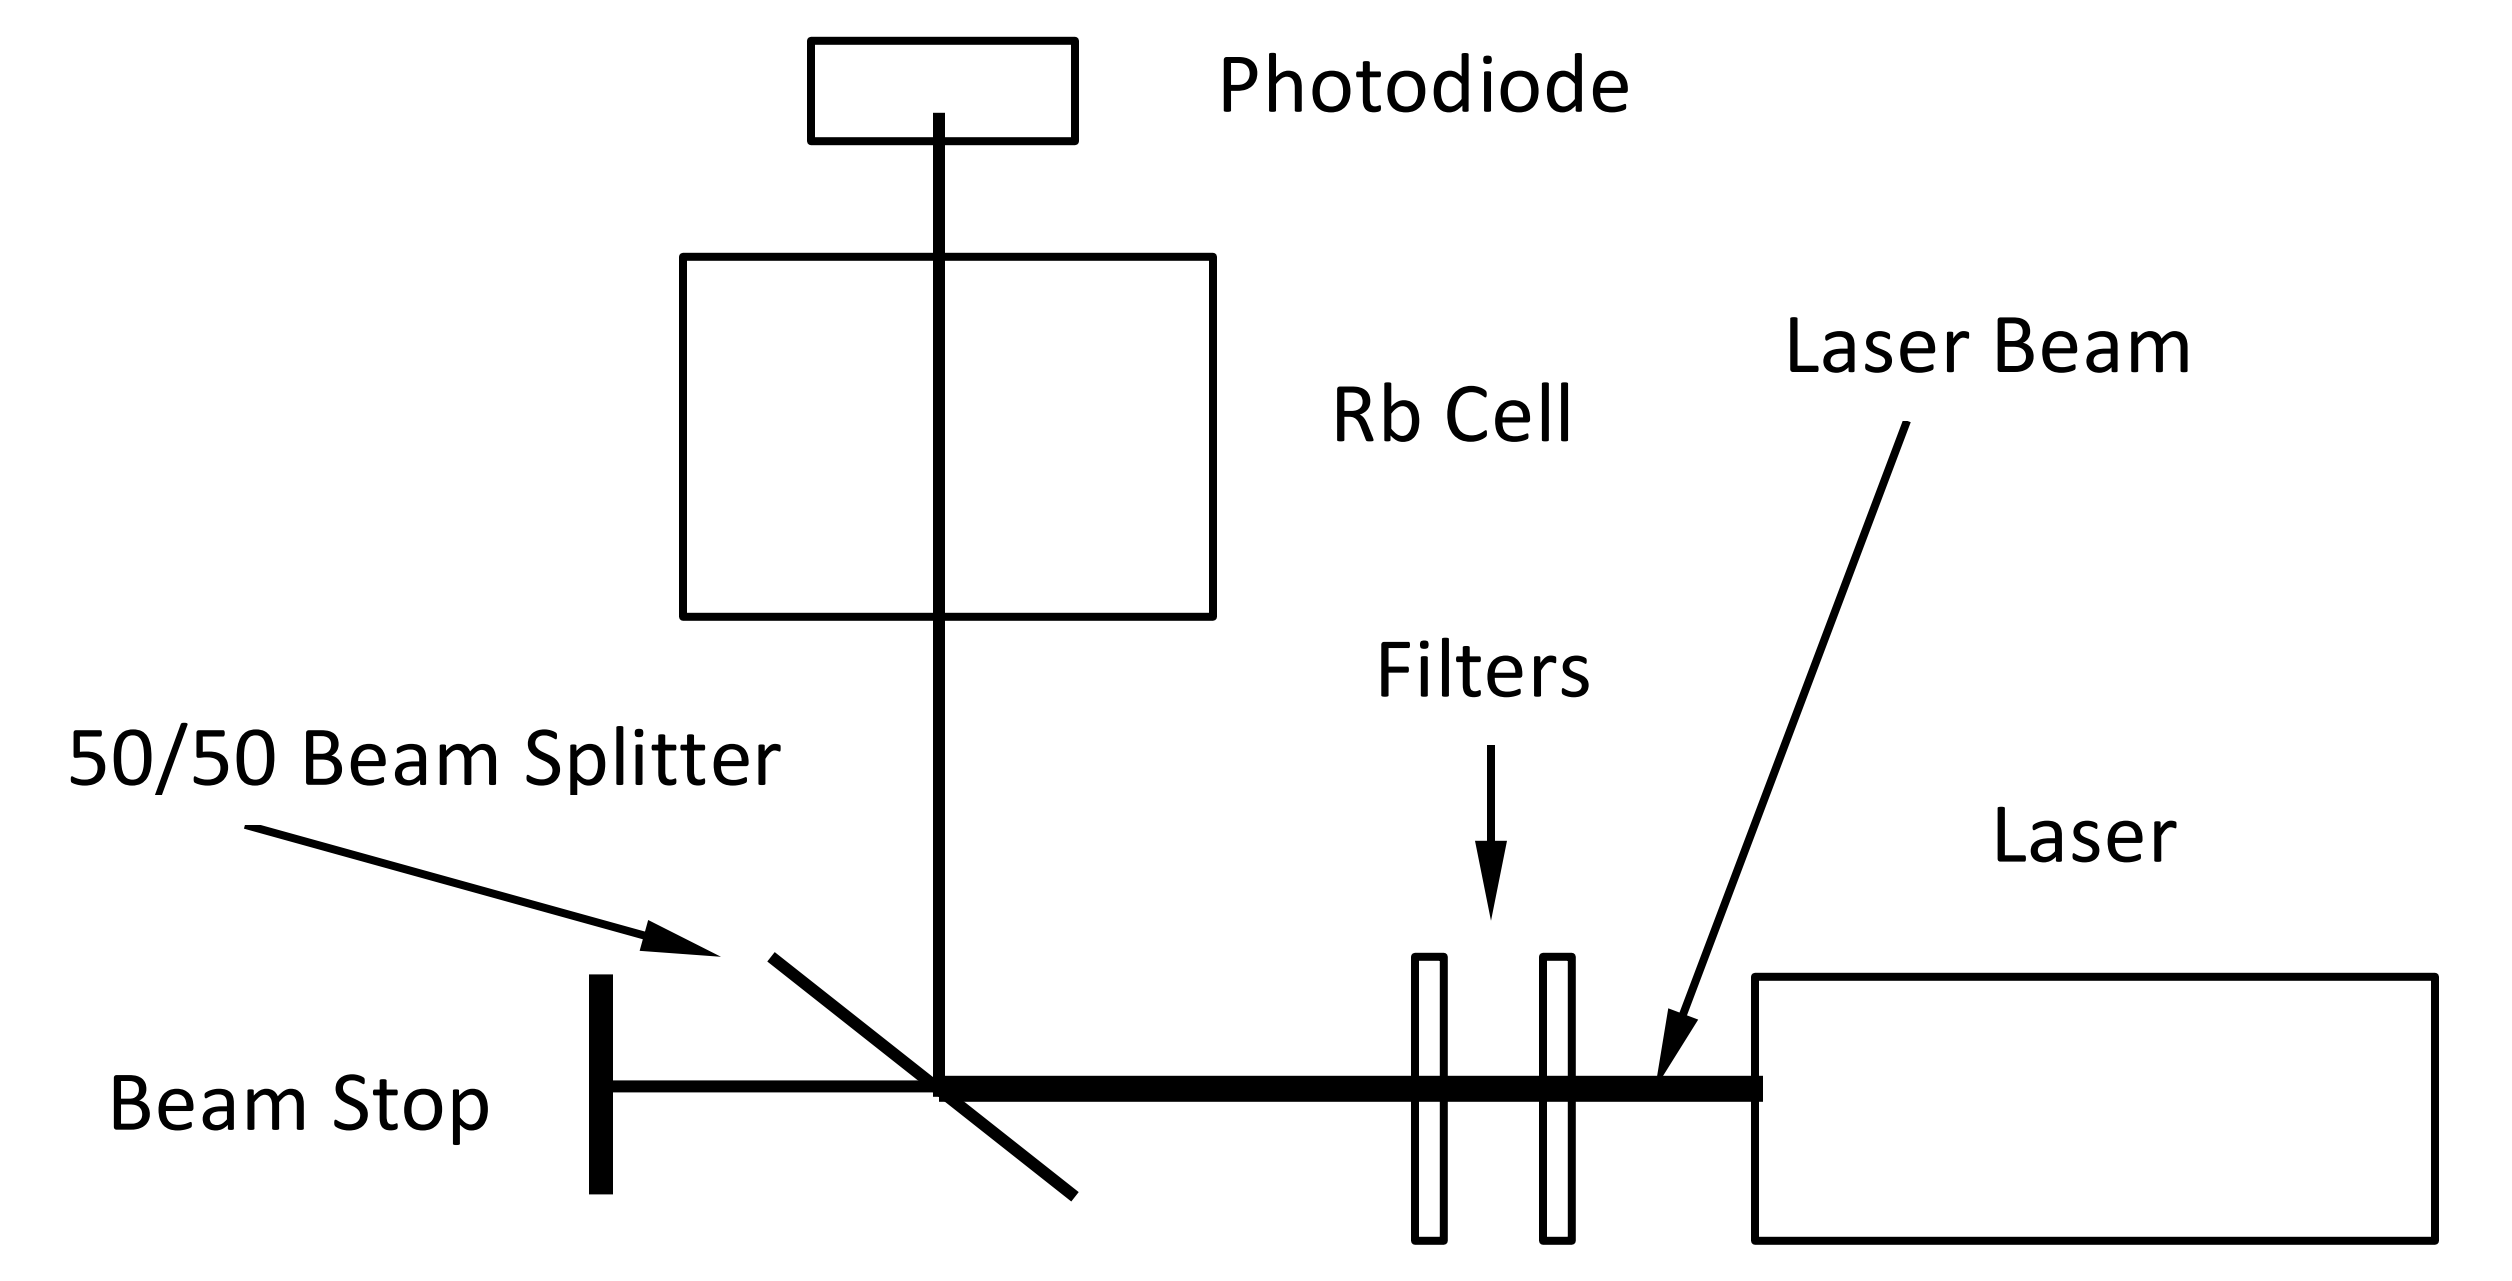
\includegraphics[width=0.4\textwidth]{Equipment/Setup1.png} \label{Setup1}}
		\qquad
		\subfloat[Diode Laser Controller hookups for \protect\cref{Setup1}]{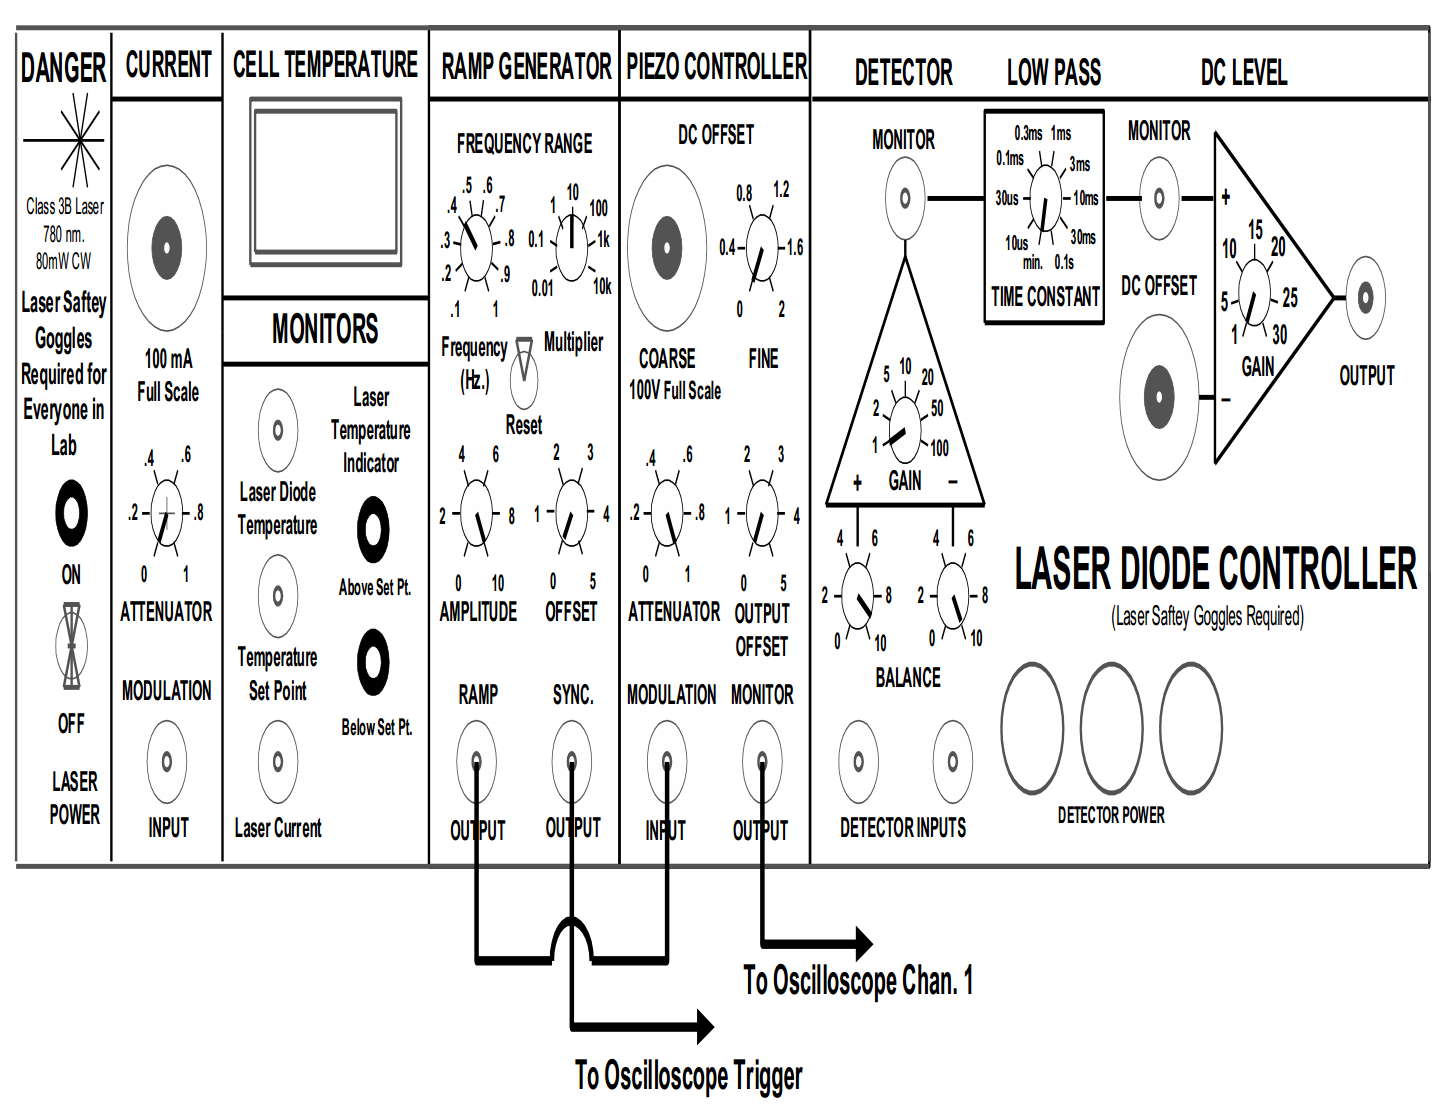
\includegraphics[width=0.4\textwidth]{Equipment/Controller1.png}}
		\caption{Optical setup and controller hook ups for measurements with mode hopping.}
		\label{Controller1}		
	\end{figure}
	
	To obtain the spectrum with the background subtracted out, we configure the optics according to \cref{Setup2} and the laser diode controller according to \cref{Controller2}. This time, the signal from photodiode $2$ is subtracted from the signal from photodiode $1$.
	
	% Setup 2
	\begin{figure}[H]
		\centering
		\subfloat[Optical setup for obtaining spectrum with background subtracted.]{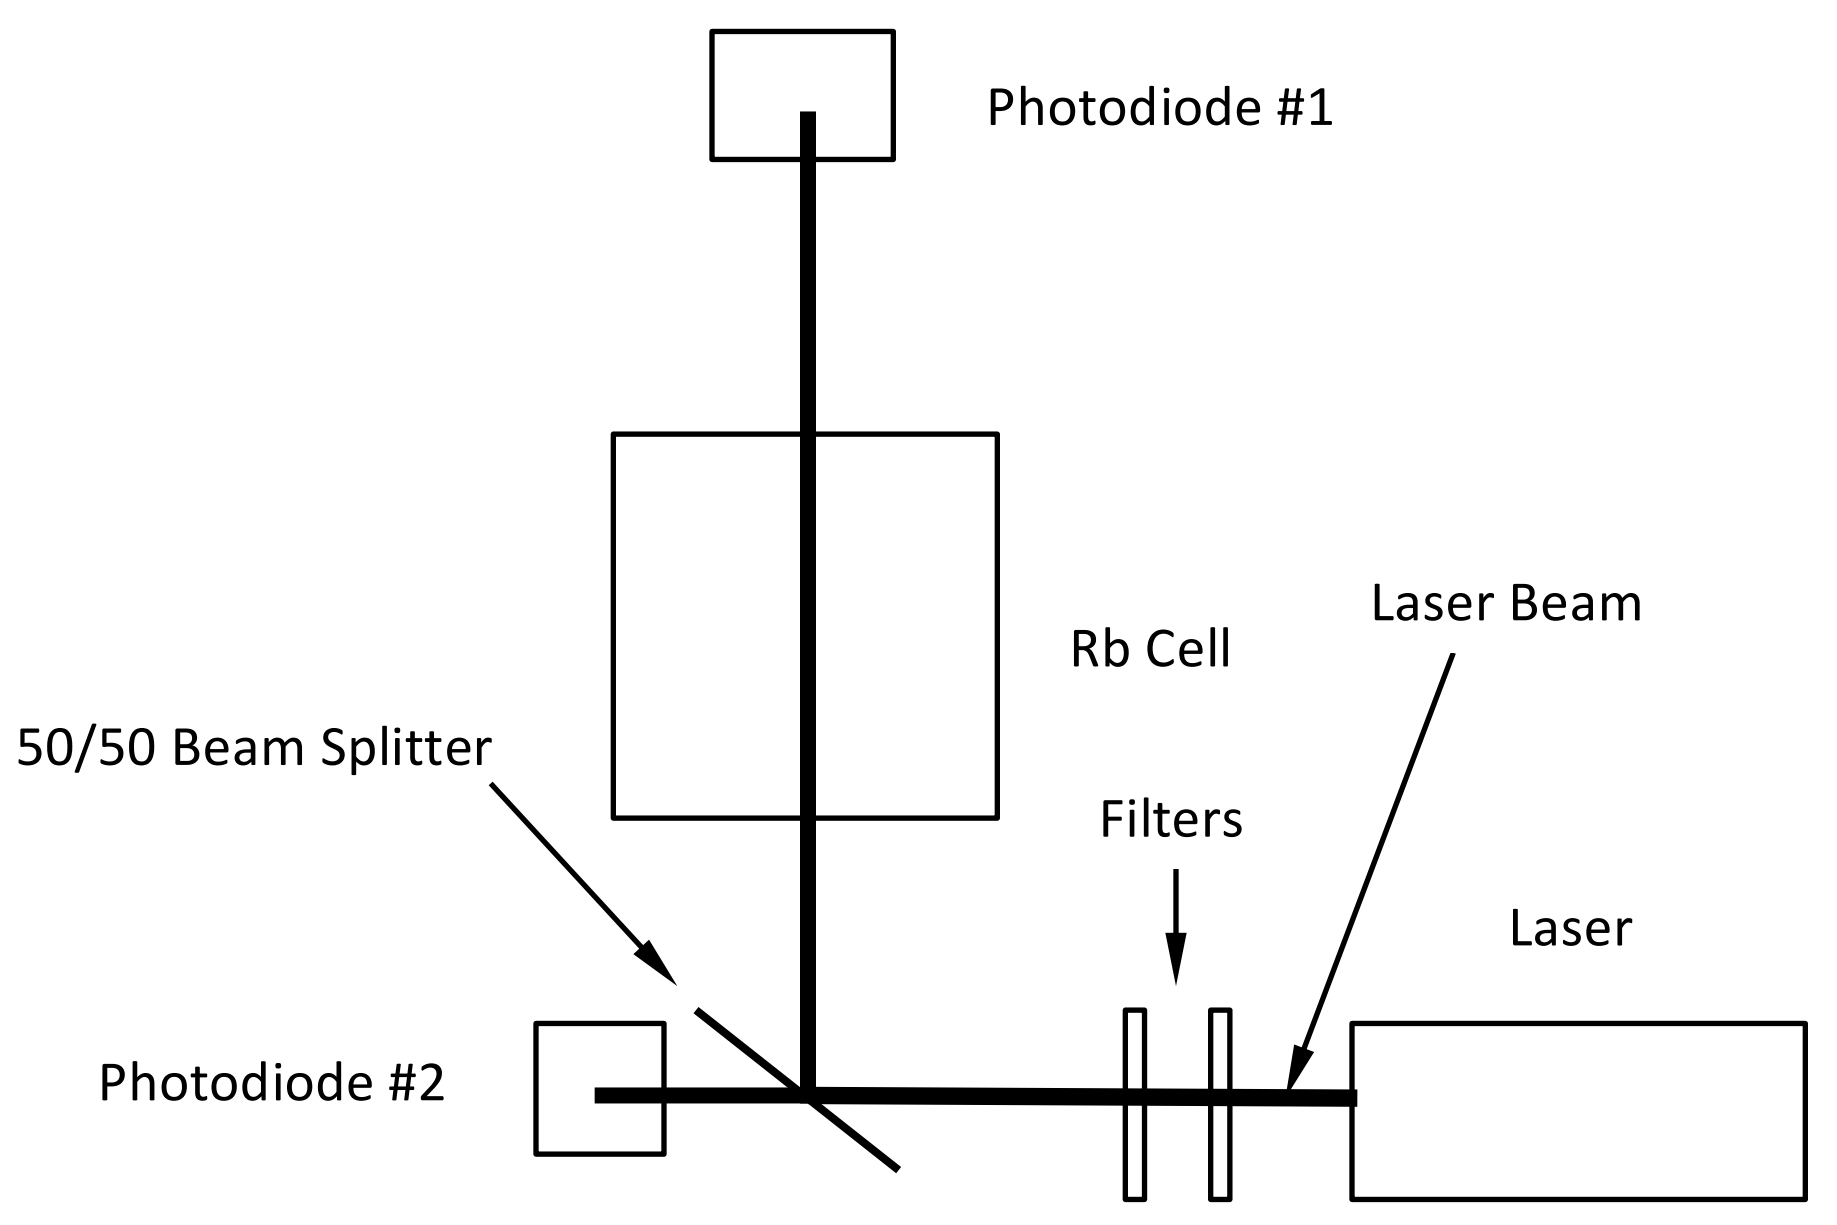
\includegraphics[width=0.4\textwidth]{Equipment/Setup2.png} \label{Setup2}}
		\qquad
		\subfloat[Diode Laser Controller hookups for \protect\cref{Setup2}] {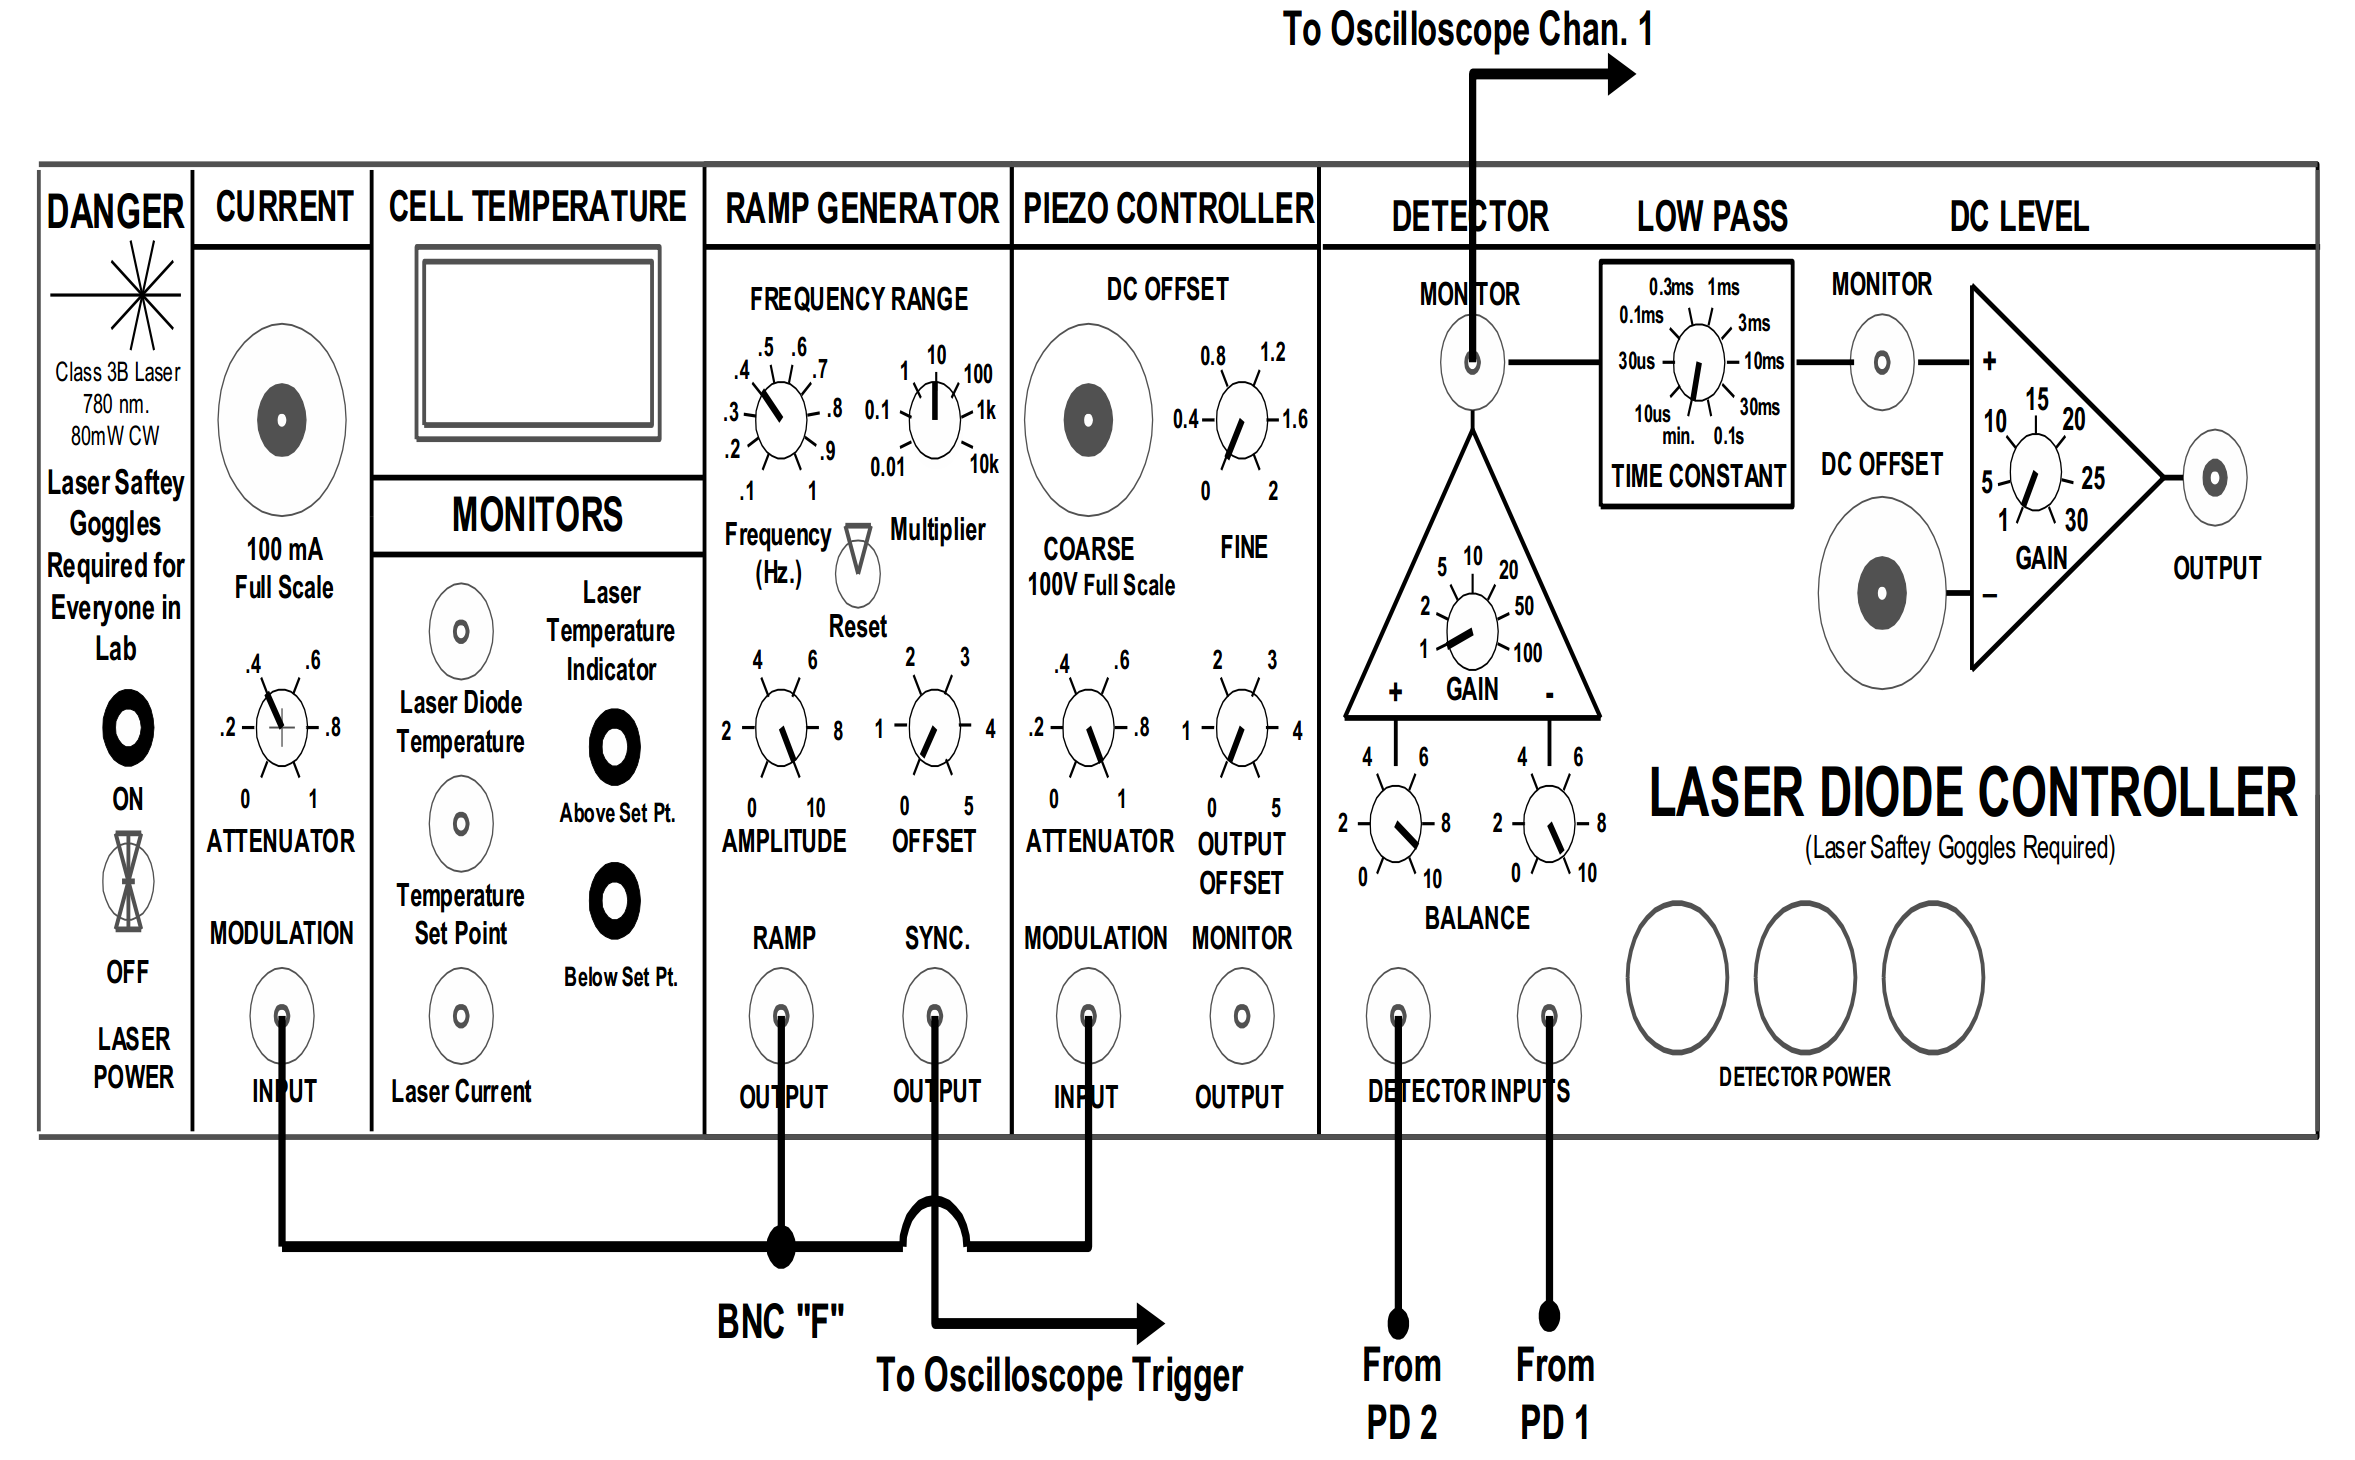
\includegraphics[width=0.4\textwidth]{Equipment/Controller2.png}\label{Controller2}}
		\caption{Laser setup and controller hookups for obtaining the spectrum with the background subtracted out}
	\end{figure}

	\pagebreak
	
	\begin{wrapfigure}{l}{0.5\textwidth}
		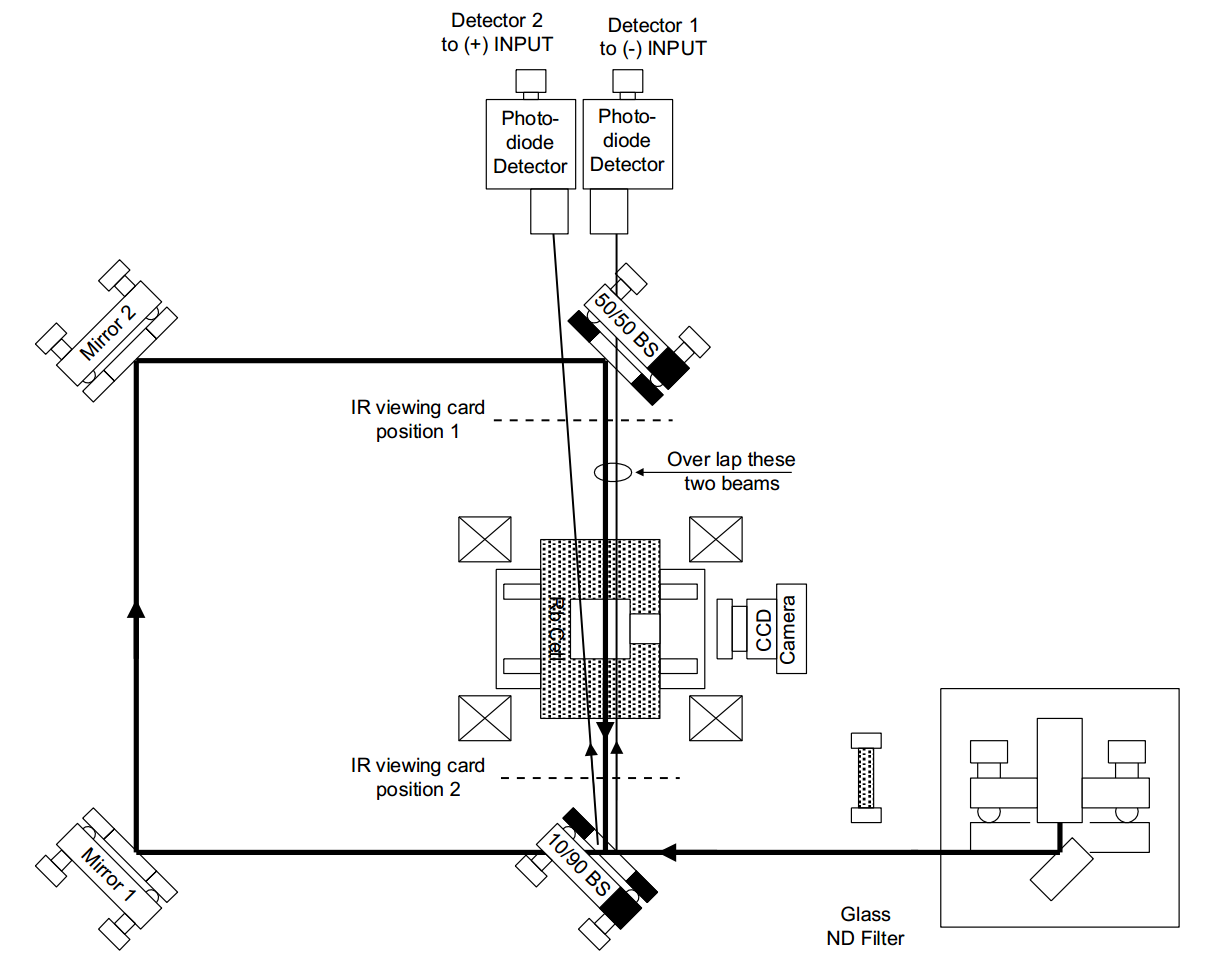
\includegraphics[width=0.5\textwidth]{/Equipment/Setup3.png}
		\caption{Optical setup for saturated absorption measurements}
		\label{Setup3}
	\end{wrapfigure}
	
	
	To obtain the hyperfine structure of the two Rubidium isotopes, we configure the laser bench according to \cref{Setup3}. In this setup, the signal from photodiode $2$ is again subtracted from photodiode $1$. This time however, the signal from photodiode $1$ is saturated, which reveals the hyperfine structure after the subtraction.
	
	When aligning the beams, two considerations must be taken into account. First, it is crucial that the beams overlap as much as possible within the absorption chamber. The larger the overlap, the sharper the higher the saturated absorption peaks will appear on the oscilloscope. Second, it is important to check that after alignment the pump beam is not being reflected off the $10/90$ beam splitter, back through the absorption cell and into either photodetector. This will result in unwanted background.
	
	
	
	\section{Results and Analysis}
		
	\begin{multicols}{2}
	\subsection{Fine Structure Spectrum}
	
% Rb Fine Spectrum
\begin{figure}[H]
	\centering
	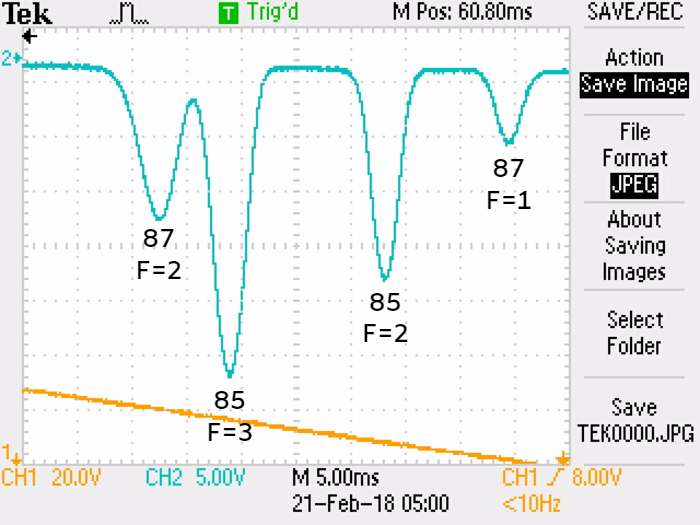
\includegraphics[width=0.45\textwidth]{Fine_Structure/AnnotatedSpectrum.jpg}
	\caption{Annotated fine structure absorption spectrum of \RbEF and \RbES}
	\label{RubidiumFineStructure}		
\end{figure}

	\columnbreak
	
	After configuring the optical bench according to \cref{Setup2}, we measured the fine structure of the Rubidium sample. An annotated spectrum is provided below in \cref{RubidiumFineStructure}. It is important to note that because the sample of Rubidium is naturally occurring, the absorption spectra of both are superimposed on each other.
	
	\end{multicols}
	
	\pagebreak
	\subsection{Hyperfine Structure Spectrum}
		
	\begin{multicols}{2}
	\begin{figure}[H]
		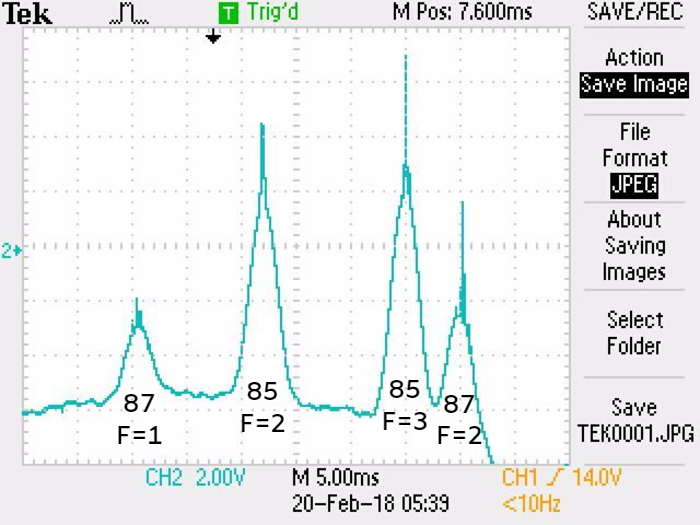
\includegraphics[width=0.45\textwidth]{Hyperfine_Structure/AnnotatedHyperFineStructureSpectrum.JPG}
		\caption{Hyperfine spectrum with background subtracted}
		\label{HyperfineStructure}
	\end{figure}
	
	\columnbreak
	
	After setting up the laser for saturated absorption, we can see a rough scan of the Hyperfine structure for both isotopes in \cref{HyperfineStructure}. The widened base is due to the imperfect subtraction of the two signals and the sharp peaks are the hyperfine transitions. \cref{85Hyper} and \cref{87Hyper} below show annotated scans of the hyperfine transitions after zooming into each peak. It is important to note the crossover resonances which lie directly in between atomic transitions. These appear to be features resulting from atomic absorption, but are generated from the process of saturated absorption spectroscopy and should be ignored.
	\end{multicols}
	
% Rb85 Hyperfine Transistions
	\begin{figure}[H]
		\centering
		\subfloat[\RbEF $F=2$ peak]
		{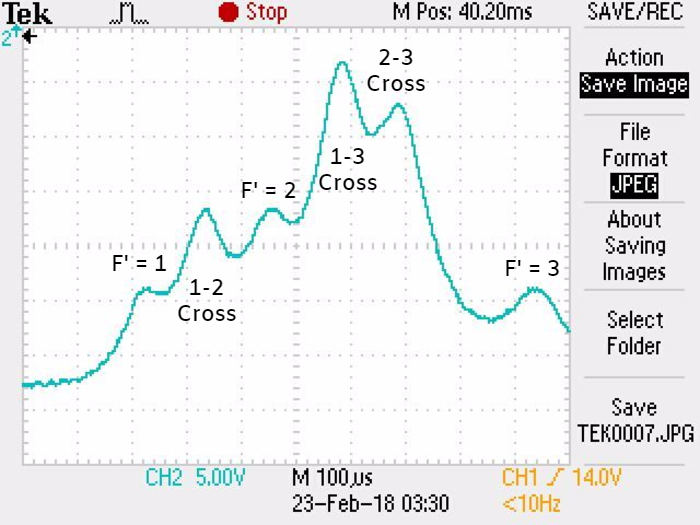
\includegraphics[width=0.4\textwidth]{Hyperfine_Structure/Peak03Annotated.JPG} \label{85aHyper}}
		\qquad
		\subfloat[\RbEF $F=3$ peak]
		{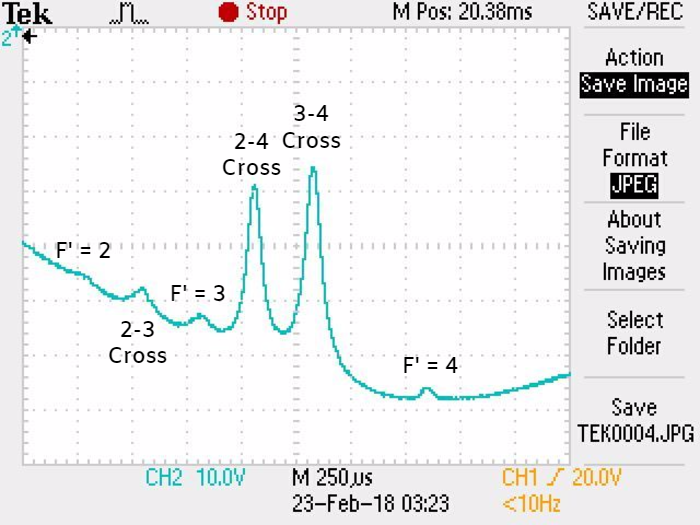
\includegraphics[width=0.4\textwidth]{Hyperfine_Structure/Peak02Annotated.JPG} \label{85bHyper}}
		\caption{Hyperfine transitions of the $^{85}\text{Rb}$-a transition \protect\subref{85aHyper} and the $^{85}\text{Rb}$-b transition \protect\subref{85bHyper}.}
		\label{85Hyper}
	\end{figure}
	
% Rb87 Hyperfine Transitions
	\begin{figure}[H]
		\centering
		\subfloat[\RbES F=1 peak]
		{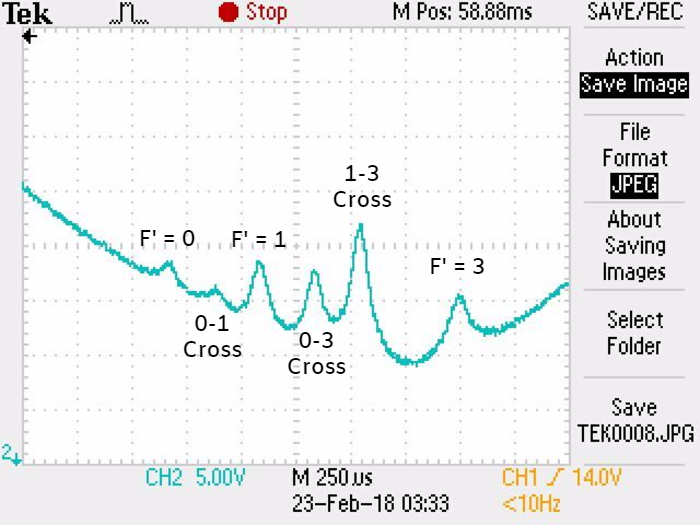
\includegraphics[width=0.4\textwidth]{Hyperfine_Structure/Peak04Annotated.JPG} \label{87aHyper}}
		\qquad
		\subfloat[\RbES F=2 peak]
		{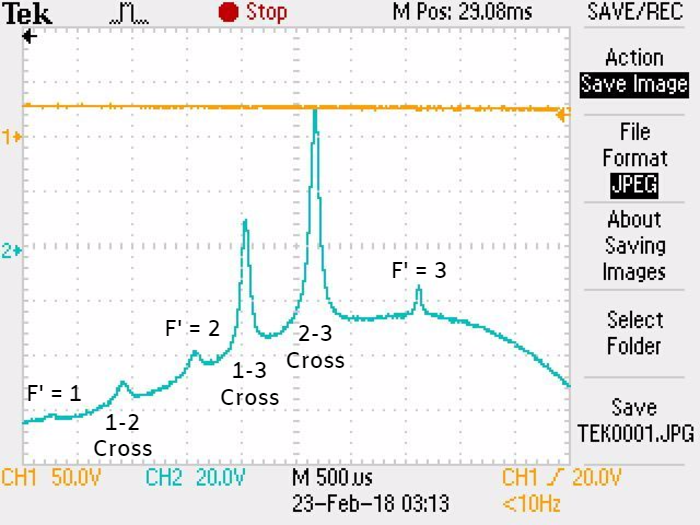
\includegraphics[width=0.4\textwidth]{Hyperfine_Structure/Peak01Annotated.JPG} \label{87bHyper}}
		\caption{Hyperfine transitions of the $^{87}\text{Rb}$-a transition \protect\subref{87aHyper} and the $^{87}\text{Rb}$-b transition \protect\subref{87bHyper}.}
		\label{87Hyper}
	\end{figure}		
		
	We provide below in \cref{EnergyLevelDiagrams}, quantitative energy level diagrams for \RbEF and $^{87}\text{Rb}$. The energies of the hyperfine transitions are summarized in \cref{Rb85Table,Rb87Table}
	
% Rb85 Level Diagram
	\begin{figure}[H]
		\centering
		\subfloat[Energy level diagram for \RbEF]{
		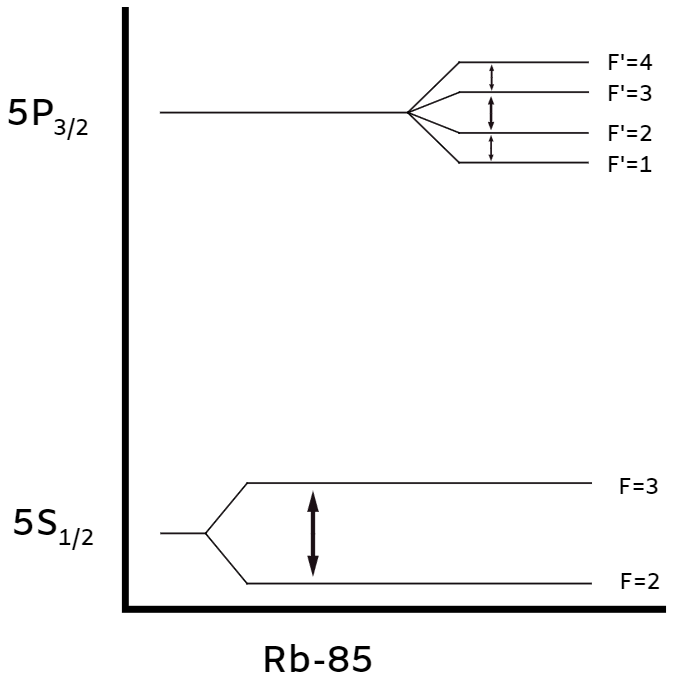
\includegraphics[width=0.45\textwidth]{LevelDiagrams/Rb85LevelDiagram.png} \label{Rb85Levels}}
		\qquad
		\subfloat[Energy level diagram for \RbES]{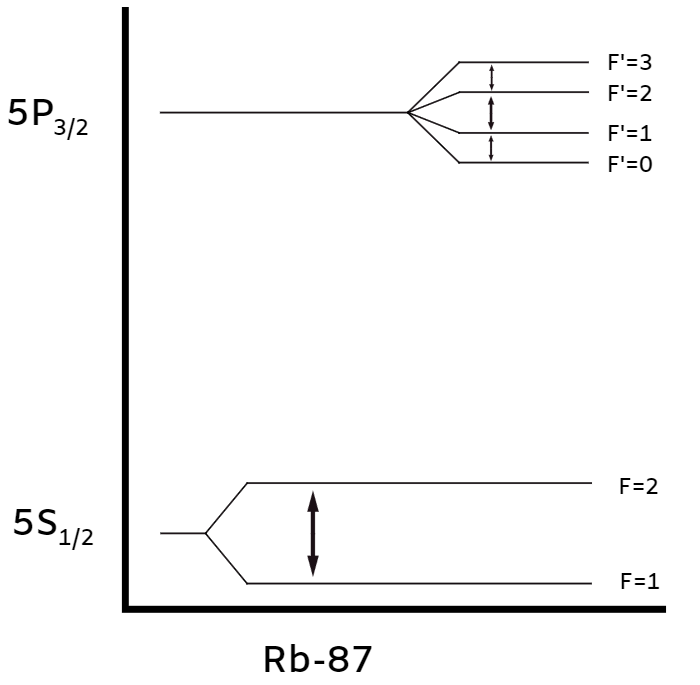
\includegraphics[width=0.45\textwidth]{LevelDiagrams/Rb87LevelDiagram.png} \label{Rb87Levels}}
		\caption{Energy level diagrams for \RbEF and \RbES.}
		\label{EnergyLevelDiagrams}
	\end{figure}


% Rb85 Table
	\begin{table}[H]
	\centering
	\begin{tabular}{c c c c}
		\toprule
		\textbf{Transition} & \textbf{Frequency (MHz)} & \textbf{Uncertainty (MHz)}  \\ \midrule
		$F'=4\rightarrow F'=3$ & $242$  & $\pm 26.3$ \\
		$F'=3\rightarrow F'=2$ & $114$  & $\pm 26.3$ \\
		$F'=2\rightarrow F'=1$ & $55.0$ & $\pm 26.3$ \\
		$F=3 \rightarrow F=2$  & $3320$ & $\pm 117$  \\
		\bottomrule
	\end{tabular}
	\caption{Table of transition energies for \RbEF corresponding to \cref{Rb85Levels}}
	\label{Rb85Table}
\end{table}

% Rb87 Table
	\begin{table}[H]
	\centering
	\begin{tabular}{c c c c}
		\toprule
		\textbf{Transition} & \textbf{Frequency (MHz)} & \textbf{Uncertainty (MHz)}  \\ \midrule
		$F'=1 \rightarrow F'=0$ & $94.8$ & $\pm 29.3$ \\
		$F'=2 \rightarrow F'=1$ & $281$  & $\pm 58.5$ \\
		$F'=3 \rightarrow F'=2$ & $462$  & $\pm 58.5$ \\
		$F=2 \rightarrow F=1$   & $7390$ & $ \pm 117$ \\ 
		\bottomrule
	\end{tabular}
	\caption{Table of transition energies for \RbES corresponding to \cref{Rb87Levels}}
	\label{Rb87Table}
\end{table}
	
	\subsection{Zeeman Effect}
	We focus on the \RbES $F=2$ line to observe the Zeeman splitting. Zeeman splitting is most easily observed in the $1-3$ crossover, $2-3$ crossover, and $F'=3$ lines within the $F=2$ line. \cref{HyperFineBField} shows oscilloscope traces for the Zeeman splitting for various magnetic fields strengths. We summarize our measurements below in \cref{splittingGraph}. We can see that the Zeeman splitting is linear, which matches the functional form of \cref{zeemanWeak}.
	\begin{figure}[H]
		\centering
		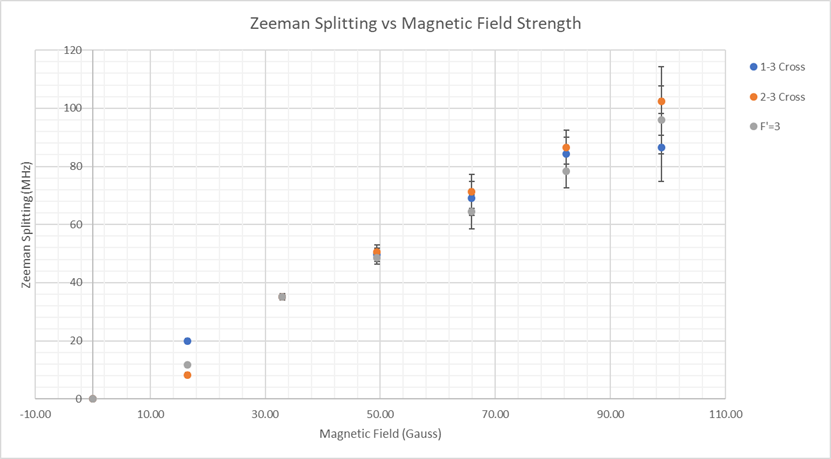
\includegraphics[width=0.8\textwidth]{HyperFineBField/SplittingGraph.png}
		\caption{Zeeman splitting for the transition peaks within the $F=2$ peak of \RbES.}
		\label{splittingGraph}
	\end{figure}
	
	
	\begin{table}[H]
		\centering
		\begin{tabular}{c c c c c c}
			\toprule
			\textbf{$|\mathbf{B}|$ (G)} & \textbf{$\Delta |\mathbf{B}|$ (G)} & \textbf{$\mathbf{1-3}$ (MHz)} & \textbf{$\mathbf{2-3}$ (MHz)} & $\mathbf{F'=3}$ \textbf{(MHz)} & \textbf{$\mathbf{\Delta f}$ (MHz)} \\ \midrule
			0    & $\pm$0     & 0    & 0    & 0    & $\pm$0 \\ 
			16.5 & $\pm$0.330 & 20.0 & 8.19 & 11.7 & $\pm$0.467 \\ 
			33.0 & $\pm$0.330 & 35.1 & 35.1 & 35.1 & $\pm$1.17 \\ 
			49.4 & $\pm$0.330 & 49.6 & 50.5 & 48.7 & $\pm$2.34 \\
			65.9 & $\pm$0.330 & 69.0 & 71.4 & 64.4 & $\pm$5.85 \\
			82.4 & $\pm$0.330 & 84.2 & 86.6 & 78.4 & $\pm$5.85 \\
			98.9 & $\pm$0.330 & 86.6 & 102  & 95.9 & $\pm$11.7 \\ \bottomrule
		\end{tabular}
	\caption{Data table summarizing the Zeeman splitting for the $F=2$ peak of \RbES at various magnetic field strengths.}
	\end{table}

	\subsection{Land\'e g-factor}
	Using the first order approximation for Zeeman splitting,  \cref{zeemanWeak}, and data measured for the $F'=3$ hyperfine transition of \RbES, we determine $g_F$ which is summarized in \cref{LandeTable}.

	\begin{table}[H]
		\centering
		\begin{tabular}{c c c c c} 
			\toprule
			$\mathbf{f}$ \textbf{(MHz)} & $\mathbf{E}$ \textbf{(Erg)} & $\mathbf{|B|}$ \textbf{(G)} & $\mathbf{g_F}$ & $\bm{\Delta} \mathbf{g_F}$  \\ \midrule
			11.7 & 7.75 $\times 10^{-20}$ & 16.5 & 0.254 & $\pm 0.0203$ \\
			35.1 & 2.33 $\times 10^{-19}$ & 33.0 & 0.381 & $\pm 0.0152$ \\
			48.7 & 3.22 $\times 10^{-19}$ & 49.4 & 0.352 & $\pm 0.00938$ \\
			64.4 & 4.26 $\times 10^{-19}$ & 65.9 & 0.349 & $\pm 0.00689$ \\
			78.4 & 5.19 $\times 10^{-19}$ & 82.4 & 0.340 & $\pm 0.00544$ \\
			95.9 & 6.36 $\times 10^{-19}$ & 98.9 & 0.347 & $\pm 0.00462$ \\
			&            & \textbf{Average} & $\mathbf{0.337}$ & $\mathbf{\pm 0.0301}$ \\ \bottomrule
		\end{tabular} 
		\caption{Table of values used to calculate $g_F$}
		\label{LandeTable}
	\end{table}
	
	
	\section{Conclusion}
	
	\subsection{Accomplishments}
	In this experiment, we successfully measured the fine structure splitting, hyperfine splitting, and Zeeman splitting between the ground state and the first excited state of \RbEF and $^{87}\text{Rb}$. For \RbEF and \RbES, we measure $\Delta E = 3320 \pm 117$ Hz and $\Delta E = 7930 \pm 117$ Hz. We also measure the hyperfine splitting for each isotope, summarized in \cref{Rb85Table,Rb87Table}. The Zeeman splitting measurements are recorded for the $F'=3$ peak within the $F=2$ peak of $^{87}\text{Rb}$. Finally, we measure the value of the Land\'e g-factor to be $g=0.337 \pm 0.0301$.
	
	\subsection{Error}

	Due to time constraints, we were unable to perform the frequency calibration of the laser ourselves. It appears as if our energy measurements for the hyperfine splitting are about twice too high compared to the accepted values. One obvious reason could be due to quoting an incorrect calibration value. 
	
	When determining the transition energies, I printed oscilloscope traces and measured frequency differences by hand, unaided by a computer program. This introduced unneeded human error into the measurements. A better method utilizes computer image manipulation software like ImageJ to make precise measurements digitally.
	
	While measuring the magnetic field, it became very difficult to follow specific transition lines as the magnetic field increased. We suspect that in part, this is due to the poor quality of the oscilloscope. The trigger level was far too sensitive for fine adjustments and the oscilloscope trace was constantly fluctuating around the screen making it hard to follow specific peaks. To fix this, a higher quality oscilloscope is required.
	
	\subsection{Extensions} 
	Spectroscopy has many useful applications in astronomy.	For planets with atmospheres that pass in front of a star, the chemical composition of the atmosphere may be determined using a spectroscopic decomposition similar to this experiment.
	
	Saturated absorption spectroscopy allows signals ``hidden'' within a doppler-broadened peak to be resolved with fine detail. This technique can be applied measure the fine structure, and hyperfine structure constants.
	
	\newpage
	\section*{Appendix}

\subsection*{Resistor Dependence}

\begin{table}[H]
	\centering
	\begin{tabular}{l l c c} \toprule
		\textbf{R} $\mathbf{[\Omega]}$ & $\mathbf{\delta R \ [\Omega]}$ & \textbf{S [W]}   & $\mathbf{\delta S \ [W]}$  \\ \toprule
		10      & 0.04 & 6.43E-17 & 1.34E-17 \\
		100     & 0.4  & 6.72E-17 & 1.28E-17 \\
		1000    & 4    & 8.08E-17 & 1.07E-17 \\
		10000   & 40   & 2.33E-16 & 1.85E-16 \\
		100000  & 400  & 1.74E-15 & 2.29E-17 \\
		1000000 & 4000 & 1.18E-14 & 1.19E-16 \\
		\bottomrule  
	\end{tabular}
	\caption{Table of measured values for resistance and power for Johnson noise}
	\label{johnsonRTable}
\end{table}

\subsection*{Temperature Dependence Data}
The following graph shows the conversion between voltage and absolute temperature. The data is provided in the laboratory manual.

\begin{figure}[H]
	\centering
	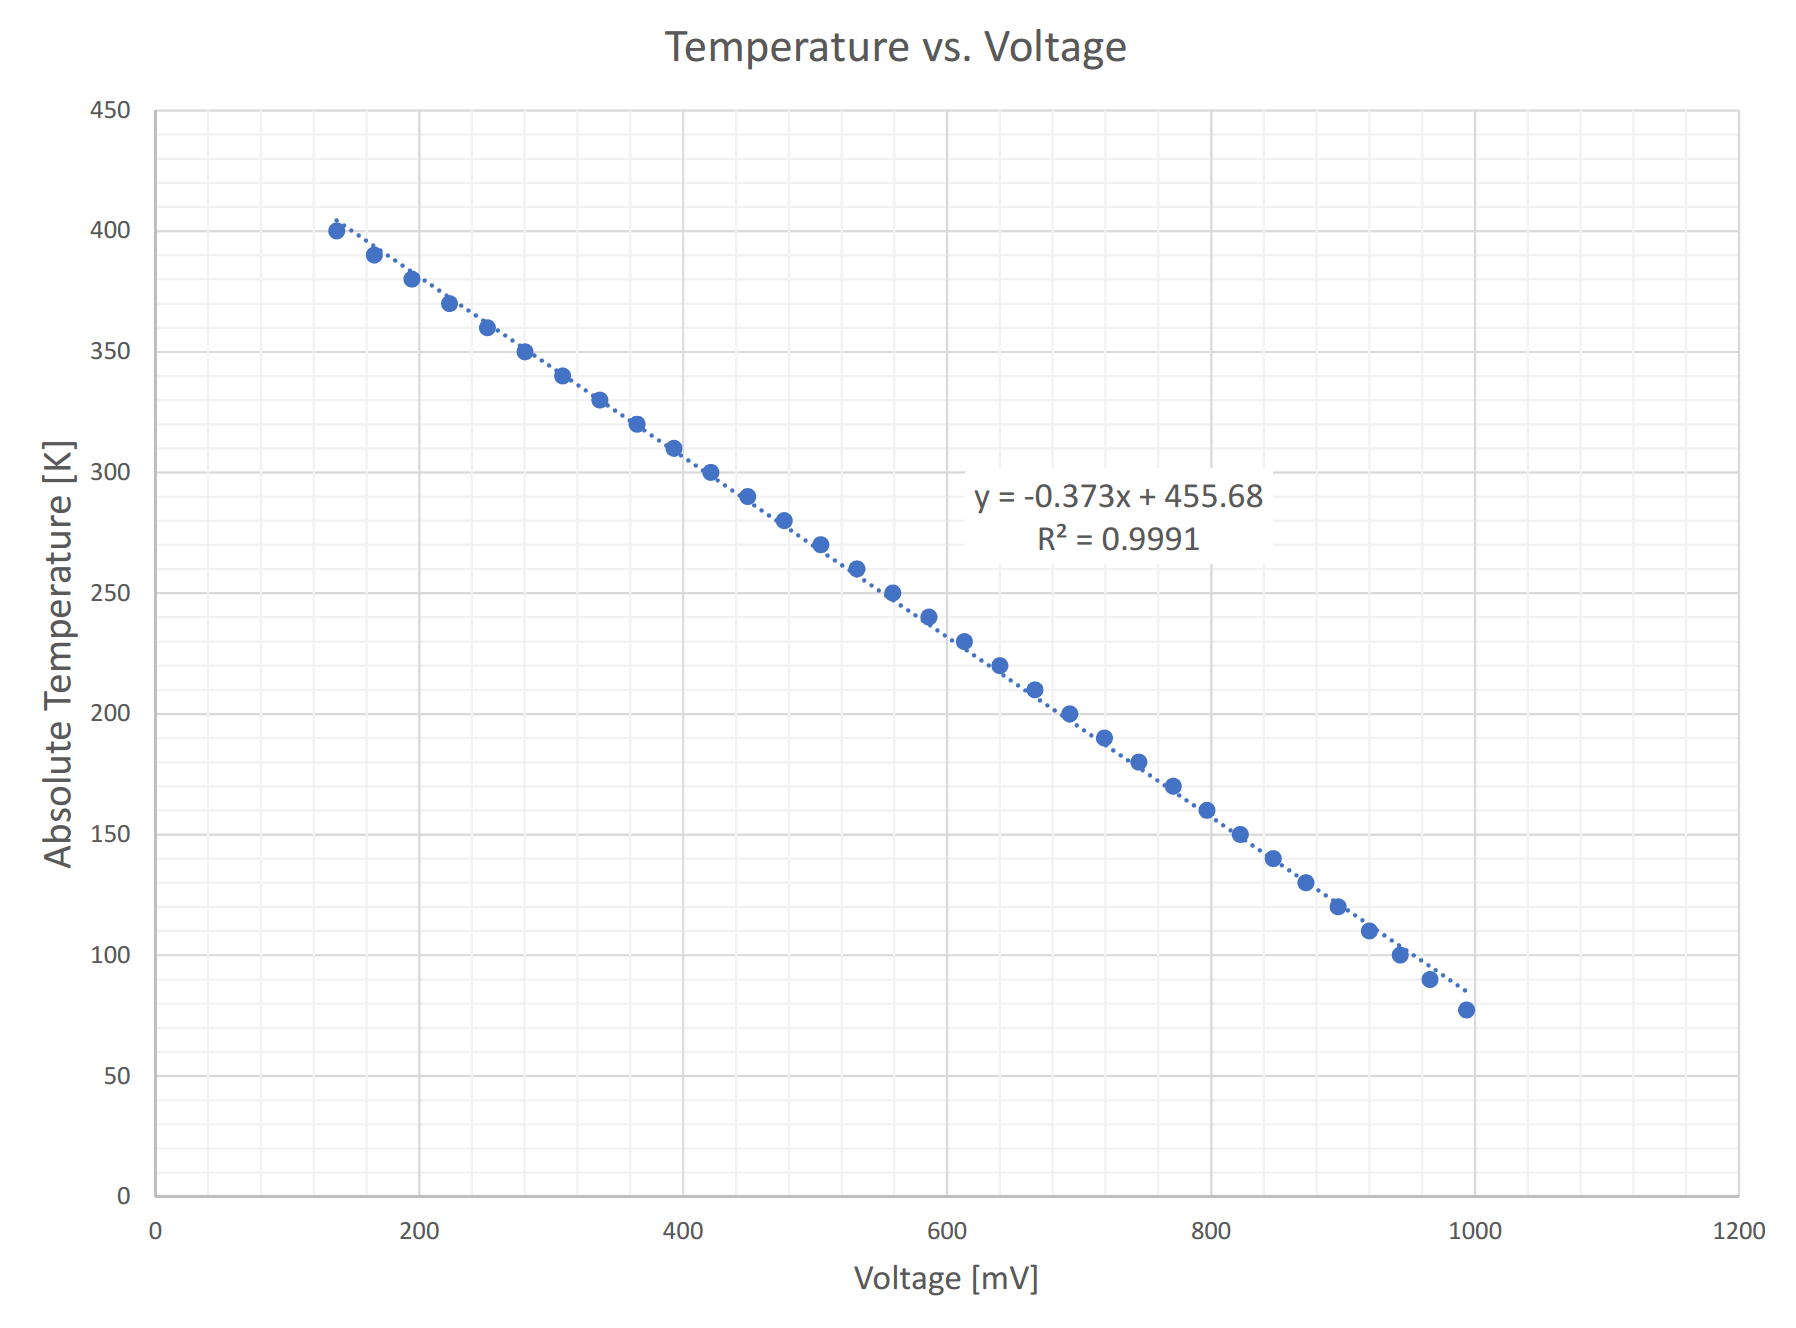
\includegraphics[width=0.7\textwidth]{TVConversion.PNG}
	\caption{Conversion between voltage and absolute temperature for a photodiode at constant $10 \ \mu A$ current.}
	\label{tvgraph}
\end{figure}


\begin{table}[H]
	\centering
	\begin{tabular}{c c c c} \toprule
		\textbf{Temp [K]} & $\mathbf{\delta}$\textbf{T [K]} & \textbf{Power [W]} & $\mathbf{\delta}$\textbf{S} \\ \toprule
		98.7 & 0.746 & 2.94E-18 & 1.29E-17 \\
		120  & 0.746 & 3.23E-18 & 1.28E-17 \\
		139  & 0.746 & 2.94E-18 & 2.58E-17 \\
		187  & 1.49  & 3.82E-18 & 1.27E-17 \\
		236  & 1.12  & 4.11E-18 & 2.53E-17 \\
		272  & 0.746 & 4.11E-18 & 2.53E-17 \\
		305  & 0.746 & 4.11E-18 & 1.27E-17 \\
		333  & 0.746 & 4.11E-18 & 1.27E-17 \\
		\bottomrule  
	\end{tabular}
	\caption{Temperature Dependence for R = 10 $\Omega$}
	\label{temp10}
\end{table}



\begin{table}[H]
	\centering
	\begin{tabular}{c c c c} \toprule
		\textbf{Temp [K]} & $\mathbf{\delta}$\textbf{T [K]} & \textbf{Power [W]} & $\mathbf{\delta}$\textbf{S} \\ \toprule
		98.3 & 0.746 & 5.52E-17 & 7.25E-18 \\
		115  & 0.746 & 6.78E-17 & 3.27E-17 \\
		141  & 0.746 & 8.22E-17 & 1.77E-17 \\
		190  & 1.49  & 1.14E-16 & 9.77E-18 \\
		230  & 1.12  & 1.38E-16 & 2.56E-17 \\
		280  & 0.746 & 1.56E-16 & 2.36E-17 \\
		304  & 0.746 & 1.74E-16 & 1.82E-17 \\
		337  & 0.746 & 1.90E-16 & 1.71E-17 \\
		\bottomrule
	\end{tabular}
\caption{Temperature Dependence for R = 10 k$\Omega$}
\label{temp10k}
\end{table}



\begin{table}[H]
	\centering
	\begin{tabular}{cccc} \toprule
		\textbf{Temp [K]} & $\mathbf{\delta}$\textbf{T [K]} & \textbf{Power [W]} & $\mathbf{\delta}$\textbf{S} \\ \toprule
		99.5 & 0.746 & 4.91E-16 & 1.63E-17 \\
		113  & 0.746 & 5.76E-16 & 1.35E-16 \\
		143  & 0.746 & 7.29E-16 & 5.49E-17 \\
		192  & 1.49  & 1.03E-15 & 4.86E-17 \\
		226  & 1.12  & 1.19E-15 & 1.82E-17 \\
		286  & 0.746 & 1.42E-15 & 2.72E-17 \\
		301  & 0.746 & 1.53E-15 & 1.63E-17 \\
		340  & 0.746 & 1.70E-15 & 2.98E-17 \\
		\bottomrule
	\end{tabular}
	\caption{Temperature Dependence for R = 100 k$\Omega$}
	\label{temp100k}
\end{table}


\subsection*{Shot Noise}

\begin{table}[H]
	\centering
	\begin{tabular}{cccc} \toprule
		$\mathbf{\Delta f}$ & $\mathbf{\delta (\Delta f)}$ & $\mathbf{\langle s \rangle}$ & $\mathbf{\delta \langle s \rangle}$ \\ \toprule
		314   & 12.56   & 9.68E-21 & 4.33E-22 \\
		984   & 39.36   & 1.97E-20 & 8.80E-22 \\
		3284  & 131.36  & 5.23E-20 & 2.34E-21 \\
		9984  & 399.36  & 1.42E-19 & 6.33E-21 \\
		32984 & 1319.36 & 4.60E-19 & 2.06E-20 \\
		99984 & 3999.36 & 1.38E-18 & 6.18E-20 \\
		\bottomrule
	\end{tabular}
	\caption{Data collected for power spectral density versus bandwidth for shot noise}
	\label{shotBandwidthTable}
\end{table}


\begin{table}[H]
	\centering
	\begin{tabular}{cccc} \toprule
		$\mathbf{I_{dc}}$ & $\mathbf{\delta (I_{dc})}$ & $\mathbf{\langle s \rangle}$ & $\mathbf{\delta \langle s \rangle}$ \\ \toprule
		1.00E-06 & 2.00E-07 & 3.21E-26 & 6.66E-27 \\
		2.00E-06 & 2.00E-07 & 9.62E-26 & 1.10E-26 \\
		3.00E-06 & 2.00E-07 & 1.16E-25 & 1.02E-26 \\
		4.00E-06 & 4.00E-07 & 1.48E-25 & 1.70E-26 \\
		5.00E-06 & 1.00E-07 & 1.76E-25 & 1.06E-26 \\
		6.00E-06 & 1.00E-07 & 2.00E-25 & 1.18E-26 \\
		7.00E-06 & 1.00E-07 & 2.44E-25 & 1.43E-26 \\
		8.00E-06 & 2.00E-07 & 2.80E-25 & 1.73E-26 \\
		9.00E-06 & 2.00E-07 & 3.17E-25 & 1.92E-26 \\
		1.00E-05 & 2.00E-07 & 3.65E-25 & 2.19E-26 \\
		\bottomrule
	\end{tabular}
	\caption{Data collected for power spectral density versus photodiode current for shot noise}
	\label{shotCurrentTable}
\end{table}
%	
	\newpage
	\bibliographystyle{utphys}
	\bibliography{references}
	\nocite{*}
	
	
\end{document}